\documentclass[10pt,t]{beamer}

\usetheme[numbering=fraction,background=light]{metropolis}

\usepackage{appendixnumberbeamer}

\usepackage{amsfonts}
\usefonttheme[onlymath]{serif}

\usepackage{booktabs}
\usepackage[scale=2]{ccicons}
\usepackage{multirow}
\usepackage{MnSymbol}
\usepackage{pgfplots}
\usepackage{pgfplotstable}
\usepackage{filecontents}
\usepackage{neuralnetwork}
\usepackage{fontspec}

\usetikzlibrary{arrows,
                arrows.meta,
                angles, 
                bending,
                intersections, 
                quotes, 
                shapes.geometric, 
                datavisualization,
                decorations.text,
                shadows}
\usepgfplotslibrary{patchplots}
\usepgfplotslibrary{dateplot}
\usepackage{kotex}
\usepackage{xspace}
\newcommand*{\Scale}[2][4]{\scalebox{#1}{\ensuremath{#2}}}%

\newfontfamily\looney[]{That's Font Folks!}
\definecolor{darkblueOuter}{RGB}{1,11,23}
\definecolor{darkblueInner}{RGB}{1,18,37}


\newcommand\blfootnote[1]{%
  \begingroup
  \renewcommand\thefootnote{}\footnote{\hspace{-0.5em}\hangindent=1.1em $\dagger$~#1}%
  \addtocounter{footnote}{-1}%
  \endgroup
}

\setbeamertemplate{frame footer}{\insertshorttitle,  ~\insertshortauthor~(\insertshortinstitute)}




\title{Math for AI}
\subtitle{A.K.A. 인공지능을 위해 꼭 필요한 것만 고른 수학}
\date{\today}
\author{Seongjin Lee}
\institute{Gyeongsang National University}

%\titlegraphic{\hfill\includegraphics[height=1.5cm]{logo.eps}}

\begin{document}

\maketitle

\begin{frame}{Table of contents}
  \setbeamertemplate{section in toc}[sections numbered]
  \tableofcontents[hideallsubsections]
\end{frame}

\section{기초}

\begin{frame}[fragile]{변수와 상수}
    \begin{columns}[T,onlytextwidth]
        \column{0.60\textwidth}
        \begin{enumerate}
            \item 변수(variable)는 비어있는 상자와 같아서 기본적으로 한 번의 한 가지 정보를 저장할 수 있음
            \item 상수(constant)는 고정된 값으로 한 번 정해지면 변하지 않음
        \end{enumerate}

        \begin{equation*}
        y=(x-2)/(2x+1)
        \end{equation*}    
        
        학습할 때 가중치는 변수로서 계속 변하지만, 학습이 완료된 후 모델에서 사용될 때는 상수의 역할을 함
        \column{0.40\textwidth}

        \begin{figure}
            \begin{tikzpicture}[scale=1]
                \begin{axis}[axis lines=middle]
                \addplot[smooth,domain=-4:-8/11,purple,very thick] {(x-2)/(2*x+1)};
                \addplot[smooth,domain=-2/7:4,purple,very thick] {(x-2)/(2*x+1)};
                \end{axis}
            \end{tikzpicture}
        \end{figure}
    \end{columns}

\end{frame}

\begin{frame}[fragile,allowframebreaks]{1차식과 2차식}
\begin{description}
    \item[항] 숫자나 문자, 또는 그 둘의 곲으로 표현 되는 식 \\
              예: $3, 3a, -4ab, \frac{x}{3}, a^{2}$
    \item[차수] 각 항에 변수가 곱해진 횟수. 이 때 상수만 곱해진 항은 차수가 0 (예: 3이라는 항은 차수가 0)\\ 
               $-4ab$는 $a$의 차수 1과 $b$의 차수의 합으로 2, $a^{2}$의 차수는 2
    \item[계수] 각 항에서 문자(변수)를 제외한 부분 \\(예: 3이라는 항에서 계수는 3, 
               $\frac{x}{3}$은 $\frac{1}{3}\times x$이므로 계수는 $\frac{1}{3}$)
    \item[단항식] 1개의 항으로 이루어진 식 
    \item[다항식] 여러 항이 덧셈이나 뺄셈으로 연결된 식\\
               $3a-2b +4a^{2}b+6$\\
               계수는 순서대로 $3, -2, 4, 6$, \\
               차수는 순서대로 $1, 1, 3, 0$
    \item[최고차항] 다항식에서 차수가 가장 높은 항. 최고차항이 다항식의 차수가 됨
    \item[x의 1차식] 수식의 항 중에서 최고차항의 차수가 1인 식 
    \item[절편] $x=0$일 때 $y$의 값
    \item[기울기] $y=ax+b$에서 계수 $a$. x의 증가 속도를 나타냄
    \begin{columns}
        \column{0.45\textwidth}
        \begin{figure}
            \begin{tikzpicture}[scale=0.5]
                \begin{axis}[axis lines=middle]
                \addplot[smooth,domain=-2:2,red,very thick] {x+1};
                \end{axis}
            \end{tikzpicture}
            \caption{$a>0$}
        \end{figure}
        \column{0.45\textwidth}
        \begin{figure}
            \begin{tikzpicture}[scale=0.5]
                \begin{axis}[axis lines=middle]
                \addplot[smooth,domain=-2:2,red,very thick] {-x+1};
                \end{axis}
            \end{tikzpicture}
        \caption{$a<0$}
        \end{figure}
    \end{columns}
    \pagebreak
    \item[x의 2차식] 수식의 항 중 최고차항이 2인 식\\
    \begin{equation*}
        y=ax^2+bx+c
    \end{equation*}    
    \begin{columns}
        \column{0.45\textwidth}
        \begin{figure}
            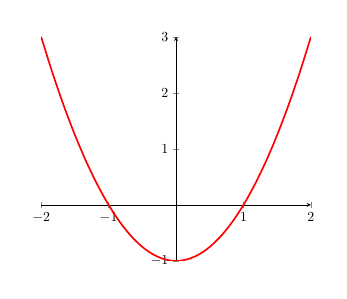
\begin{tikzpicture}[scale=0.5]
                \begin{axis}[axis lines=middle]
                \addplot[smooth,domain=-2:2,red,very thick] {x*x-1};
                \end{axis}
            \end{tikzpicture}
            \caption{$a>0$}
        \end{figure}
        \column{0.45\textwidth}
        \begin{figure}
            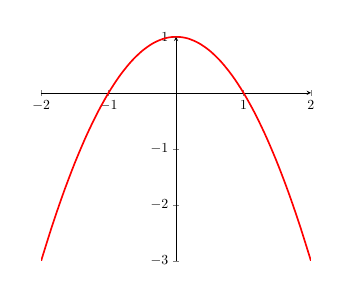
\begin{tikzpicture}[scale=0.5]
                \begin{axis}[axis lines=middle]
                \addplot[smooth,domain=-2:2,red,very thick] {-x*x+1};
                \end{axis}
            \end{tikzpicture}
        \caption{$a<0$}
        \end{figure}
    \end{columns} 
\end{description}
\end{frame}

\begin{frame}[fragile]{함수의 개념}
\begin{description}
    \item[함수] 어떤 입력값 $x$에 따라 하나의 출력값 $y$가 결정된다면 $y$는 $x$의 함수이다.  
\end{description}

\vspace{2em}
\begin{equation*}
    x \rightarrow f(x)=2x \rightarrow y
\end{equation*}

\vspace{2em}

\begin{block}{컴퓨터공학에서의 함수}
    수학의 함수보다 더 확장된 개념으로 어떤 입력 값에 대해 참이나 거짓 같은 형태 또는 문자열 같은 형태도 출력으로 사용될 수 있음
\end{block}
\end{frame}

\begin{frame}[fragile]{제곱근}
    \begin{description}
        \item[제곱근] 제곱을 했을 때 어떤 수가 되는 값을 그 어떤 수에 대한 제곱근이라고 부름. \\
        어떤 수 $a$에 대해 $a=b^2$을 만족하는 $b$가 있다면 이러한 $b$를 $a$의 제곱근이라고 함. 실수에서는 양수에 대한 제곱근이 반드시 두 개 존재함 $\pm\sqrt{a}$\\
        $\sqrt{}$ 로 표현하고 루트라고 읽음. 
    \end{description}
$a>0, b>0, c>0$일 때 다음의 식이 성립함
    \begin{enumerate}
        \item $\sqrt{a^2} = a$
        \item $a \times \sqrt{b} = a\sqrt{b}$
        \item $b\sqrt{a} + c\sqrt{a} = (b+c)\sqrt{a}$
        \item $\sqrt{a} \times \sqrt{b} = \sqrt{ab}$
        \item $\sqrt{a} \div \sqrt{c} = \frac{\sqrt{a}}{\sqrt{c}} = \sqrt{\frac{a}{c}}$
        \item $\sqrt{a^2 \times b} = a\sqrt{b}$
    \end{enumerate}
\end{frame}



\begin{frame}[fragile]{거듭제곱과 거듭제곱근}
 \begin{columns}
     \column{0.5\textwidth}
     \begin{description}
         \item[거듭제곱] $a$를 $p$번 곱한 것을 $a$의 $p$ 제곱 또는 $a$의 $p$승이라고 부르고 $a^p$라고 표기함. 
      \end{description}
      $a$를 밑수(base) $p$를 지수(exponent)라고 함. 지수는 분수 또는 음수가 될 수 있음.
      \begin{description}
        \item[거듭제곱근] $p$제곱을 하면 $a$가 되는 수를 $a$의 $p$제곱근이라고 부르고 $\sqrt[p]{a}$라고 표기함
      \end{description}
      $\sqrt[2]{a}$는 평방근이라고 부르고 2를 생략하기도 함
     \column{0.5\textwidth}
     $a>0, b>0$이라고 가정
     \begin{eqnarray*}
         a^{0} &=& 1\\
         a^p a^q &=& a^{p+q}\\
         (a^p)^q &=& a^{p+q}\\
         (ab)^p &=& a^p b^p\\
         a^{-p} &=& \frac{q}{a^p}\\
         \sqrt[p]{a}\sqrt[p]{b} &=&\sqrt[p]{ab}\\
         \sqrt[p]{\sqrt[q]{a}} &=& \sqrt[pq]{a}\\
         \sqrt[p]{a} &=& a^{\frac{1}{p}}
     \end{eqnarray*}
 \end{columns}
\end{frame}

\begin{frame}[fragile,allowframebreaks]{지수함수와 로그함수}
\begin{description}
    \item[지수함수] $a>0, a\neq 1$ 일 때 $y = a^x$와 같이 표현되는 함수 
\end{description}
\begin{columns}
    \column{0.40\textwidth}
    \begin{figure}
        \begin{tikzpicture}[scale=0.7]
            \begin{axis}[axis lines=middle]
            \addplot[smooth,domain=-2:4,purple,very thick] {1.4^x};
            \end{axis}
        \end{tikzpicture}
        \caption{$a>1$}
    \end{figure}
    \column{0.40\textwidth}
    \begin{figure}
        \begin{tikzpicture}[scale=0.7]
            \begin{axis}[axis lines=middle]
            \addplot[smooth,domain=-2:2,purple,very thick] {0.3^x};
            \end{axis}
        \end{tikzpicture}
        \caption{$0<a<1$}
    \end{figure}
    
\end{columns}

\pagebreak

\begin{description}
    \item[로그] 어떤 $x$가 $a^y$이라고 표현될 때의 지수 $y$를 $a$를 밑으로 하는 $x$의 로그라고 하며, 기호 $\log$를 사용하여 $y=\log_a^x$와 같이 표현함. 이 때, $x$를 진수(antilogarithm)라고 하는데 $a>0, a\neq1, x>0$이다.
\end{description}

$a>0, a\neq1, x, y >0$일 때 다음이 성립함
\begin{eqnarray*}
    \log_a a &= & 1 \\
    \log_a 1 &= & 0 \\
    \log_a xy &= & \log_a x + \log_a y \\
    \log_a \frac{x}{y} &= & \log_a x - \log_a y\\
    \log_a x^y &= & y\log_a x\\
    \log_a x &= & \frac{\log_c x}{ \log_c a} , c>0, c \neq 1 
\end{eqnarray*} 

\begin{description}
    \item[로그함수] 진수를 변수로 사용하는 함수. $a>0, a\neq 1, x > 0$일 때 다음과 같이 표현되는 함수를 로그함수라 함. \\
    \begin{equation*}
        y=\log_a x
    \end{equation*}  
\end{description}
\begin{columns}
    \column{0.40\textwidth}\vspace{-1em}
    \begin{figure}
        \begin{tikzpicture}[scale=0.7]
            \begin{axis}[axis lines=middle]
            \addplot[smooth,domain=0:3,purple,very thick] {ln(x)};
            \end{axis}
        \end{tikzpicture}
        \caption{$a>1$}
    \end{figure}
    \column{0.40\textwidth}\vspace{-1em}
    \begin{figure}
        \begin{tikzpicture}[scale=0.7]
            \begin{axis}[axis lines=middle]
            \addplot[smooth,domain=-2:2,purple,very thick] {ln(x)/ln(0.2)};
            \end{axis}
        \end{tikzpicture}
        \caption{$0<a<1$}
    \end{figure}
    
\end{columns}
\pagebreak

\begin{itemize}
    \item 가능성을 나타내는 척도로 우도 또는 가능도 (likelihood)를 사용하며, 가능도를 나타내는 함수를 likelihood function 가능도 함수라고함
    \item likelihood 식은 확률 식과 같고 0과 1 사이의 값을 갖음
    \item likelihood를 계속 곱하다 보면 값이 계속 작아져서 다루기 어려워짐. 그래서 likelihood와 로그 함수를 같이 사용함
    \item 로그를 사용하면 $\log_a XY = \log_a X + \log_a Y$와 같이 곱셉을 덧셈으로 표현할 수 있어서 계산이 쉬워짐
\end{itemize}
\end{frame}
    

\begin{frame}[fragile]{자연로그}
\begin{block}{자연로그의 밑, 네이피어 상수 $e$}
    \begin{equation*}
        e=\lim_{n\rightarrow\infty} \left(1+ \frac{1}{n}\right)^n = 2.718281\ldots
    \end{equation*}
    \begin{itemize}
        \item 자연상수 $e$를 사용하는 이유는 몇 가지 유용한 특징 때문임
    \end{itemize}
    \begin{eqnarray*}
        \frac{d}{dx}e^x & = & e^x\\
        \frac{d}{dx}\ln x &= &\frac{1}{x}
    \end{eqnarray*}
\end{block}
\end{frame}


\begin{frame}[fragile,allowframebreaks]{시그모이드 함수}
\begin{description}
    \item[시그모이드 함수] Sigmoid 는 다음과 같이 표현됨. \\
    \begin{equation*}
        \varsigma_a(x) = \frac{1}{1+\exp (-ax)}
    \end{equation*}
\end{description}
이 때, $a$를 게인 (gain)이라 부르는데 특별히 $a=1$일 때의 시그모이드 함수를 표준 시그모이드 함수라고 부름. $x$가 음의 무한대로 갈 때 0, 양의 무한대로 갈 때 1, 그리고 0일 때 $\varsigma_a(0)=\frac{1}{2}$가 됨

\begin{figure}
    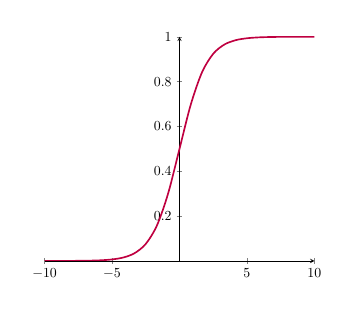
\begin{tikzpicture}[scale=0.5]
        \begin{axis}[axis lines=middle]
        \addplot[smooth,domain=-10:10,purple,very thick] {1/(1+exp(-x))};
        \end{axis}
    \end{tikzpicture}
    \caption{$a>1$}
\end{figure}
\pagebreak

다양한 활성화 함수

\begin{columns}
    \column{0.40\textwidth}
    \begin{figure}
        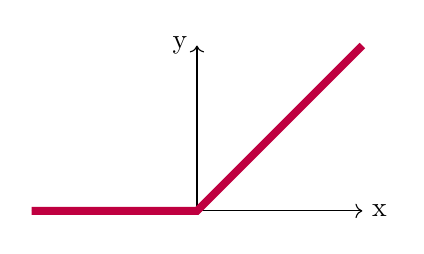
\begin{tikzpicture}[scale=0.7]
            \draw[->] (-3,0) -- (3,0) node[right] {x};
            \draw[->] (0,0) -- (0, 3) node[left] {y};
            \draw[line width = .1cm, purple]  (-3,0) -- (0,0) -- (3,3) ;
        \end{tikzpicture}
        \caption{ReLU}
    \end{figure}
    \column{0.40\textwidth}
    \begin{figure}
        \begin{tikzpicture}[scale=0.7]
            \begin{axis}[axis lines=middle]
            \addplot[smooth,domain=-5:5,purple,very thick] {tanh(x)};
            \end{axis}
        \end{tikzpicture}
        \caption{tanh 함수}
    \end{figure}
    
\end{columns}
\end{frame}
   
\begin{frame}[fragile, allowframebreaks]{삼각함수}
\begin{description}
    \item[삼각 함수] 각의 크기에 따라 값이 달라지는 함수
    \item[도수법] 원이 한 바퀴 도는 데 필요한 각을 360$^{\circ}$로 표현 
    \item[호도법] 반지름이 $r$인 원에서 그 반지름과 같은 길이의 호 $AB$가 있다고 할 때 그 중심각의 크기는 항상 일정함. 이때의 각을 1 radian이라고 부르고 1 rad라고 표기함
\end{description}

\begin{figure}
    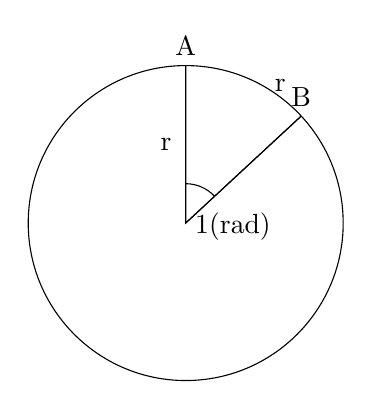
\begin{tikzpicture}[scale=0.5]
        \draw(0,0) circle [radius=4];
        \draw (0,0) -- (0, 4) node [above] {A};
        \draw (0,0) -- (2.93401886, 2.71873745) node [above] {B};
        \draw (0,4) coordinate (x) -- (0,0) coordinate (y) -- (2.93401886, 2.71873745) coordinate (z) pic [draw] {angle = z--y--x};
        \node at (-0.5,2) {r};
        \node at (2.4, 3.5) {r};
        \node[below] at (1.2,0.5) {1(rad)};
    \end{tikzpicture}
    \caption{radian}
\end{figure}

\pagebreak
\begin{table}
    \begin{tabular}{|c|c|c|c|c|c|c|c|c|} \hline
        도수법 & 0$^{\circ}$ & 30$^{\circ}$ &  45$^{\circ}$ & 60$^{\circ}$ & 90$^{\circ}$ & 120$^{\circ}$ & 180$^{\circ}$ & 360$^{\circ}$  \\ \hline
        호도법 & 0 & $\frac{1}{6}\pi$ & $\frac{1}{4}\pi$ & $\frac{1}{3}\pi$ & $\frac{1}{2}\pi$ & $\frac{2}{3}\pi$ & $\pi$ & $2\pi$ \\ \hline
    \end{tabular}
\end{table}
    \begin{columns}
        \column{0.45\textwidth}
        \begin{figure}
            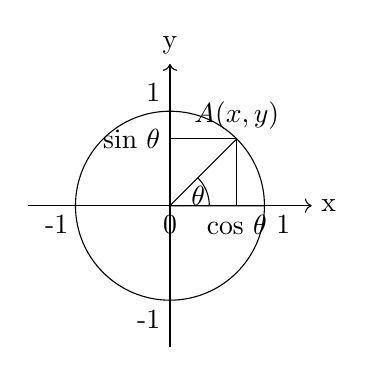
\begin{tikzpicture}[scale=1.2]
                \draw [->] (-1.5,0) -- (1.5,0) node [right] {x};
                \draw [->] (0, -1.5) -- (0, 1.5) node [above] {y};
                \draw(0,0) circle [radius=1] node [below] {0};
                \node [below] at (-1.2,0) {-1};
                \node [below] at (1.2,0) {1};
                \node [left] at (0,-1.2) {-1};
                \node [left] at (0,1.2) {1};
                \draw [-.] (0,0.7071067812) -- (0.7071067812, 0.7071067812);
                \draw [-.] (0.7071067812,0) -- (0.7071067812, 0.7071067812);
                \node [left] at (0,0.7071067812) {sin $\theta$};
                \node [below] at (0.7071067812,0) {cos $\theta$};
                \node [above] at (0.7071067812,0.7071067812) {$A(x, y)$};
                \draw (1,0) coordinate (x) -- (0,0) coordinate (y) -- (0.7071067812, 0.7071067812) coordinate (z) pic [draw] {angle = x--y--z};
                \node at (0.3, 0.1) {$\theta$};
            \end{tikzpicture}
            \caption{단위 원과 삼각함수}
        \end{figure}
    
        \column{0.45\textwidth}
        \begin{eqnarray*}
            sin\theta = y \\
            cos\theta = x \\
            tan\theta = \frac{y}{x} \\
        \end{eqnarray*}
    \end{columns}
    
\pagebreak
\begin{table}
    \begin{tabular}{|c|c|c|c|c|c|} \hline
        $\theta$ & 0 & $\frac{1}{6}\pi (=30^\circ)$ & $\frac{1}{4}\pi (=45^\circ)$ & $\frac{1}{3}\pi (=60^\circ)$ & $\frac{1}{2}\pi (=90^\circ)$ \\ \hline
        $sin\theta$ & 0 & $\frac{1}{2}$& $\frac{\sqrt{2}}{2}$& $\frac{\sqrt{3}}{2}$& $1$\\ \hline
        $cos\theta$ & 1 & $\frac{\sqrt{3}}{2}$& $\frac{\sqrt{2}}{2}$& $\frac{1}{2}$& $0$\\ \hline
        $tan\theta$ & 0 & $\frac{\sqrt{3}}{3}$& $1$& $\sqrt{3}$& -\\ \hline
    \end{tabular}
\end{table}
\begin{table}
    \begin{tabular}{|c|c|c|c|c|c|} \hline
        $\theta$ & $\frac{2}{3}\pi (=120^\circ)$ & $\frac{5}{6}\pi (=150^\circ)$ & $\pi (=180^\circ)$ & $\frac{3}{2}\pi (=270^\circ)$ & $\pi (=360^\circ)$ \\ \hline
        $sin\theta$ & $\frac{\sqrt{3}}{2}$ & $\frac{1}{2}$& 0& $-1$& $0$\\ \hline
        $cos\theta$ & $-\frac{1}{2}$ & $-\frac{\sqrt{3}}{2}$& $-1$& $0$& $1$\\ \hline
        $tan\theta$ & $-\sqrt{3}$ & $-\frac{\sqrt{3}}{3}$& $0$& $-$& $0$\\ \hline
    \end{tabular}
\end{table}

\pagebreak
\begin{itemize}
    \item 반지름 1인 원의 둘레 위의 한 점 $A$의 좌표 $x, y$는 $-1 \leq x \leq 1$과 $-1 \leq y \leq 1$ 범위 안에 있음
    \item 같은 이유로 $\sin \theta, \cos \theta$가 갖을 수 있는 값의 범위도 $-1 \leq \sin \theta \leq 1$, $-1 \leq \cos \theta \leq 1$ 이 됨
    \item $\tan \theta$는 임의의 실숫값을 갖음
    \item 함수가 값을 가질 수 있는 범위를 치역 (range)라고 함
\end{itemize}

\begin{columns}
    \column{0.3\textwidth}
    \begin{eqnarray*}
        \tan \theta = \frac{\sin \theta}{\cos \theta}\\
        \sin^2\theta + \cos^2 \theta = 1\\
        1 + \tan^2\theta = \frac{1}{\cos^2\theta}    
    \end{eqnarray*}
    \column{0.4\textwidth}\vspace{-1em}
    \begin{figure}
        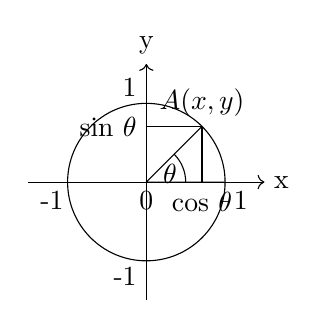
\begin{tikzpicture}[scale=1]
            \draw [->] (-1.5,0) -- (1.5,0) node [right] {x};
            \draw [->] (0, -1.5) -- (0, 1.5) node [above] {y};
            \draw(0,0) circle [radius=1] node [below] {0};
            \node [below] at (-1.2,0) {-1};
            \node [below] at (1.2,0) {1};
            \node [left] at (0,-1.2) {-1};
            \node [left] at (0,1.2) {1};
            \draw [-.] (0,0.7071067812) -- (0.7071067812, 0.7071067812);
            \draw [-.] (0.7071067812,0) -- (0.7071067812, 0.7071067812);
            \node [left] at (0,0.7071067812) {sin $\theta$};
            \node [below] at (0.7071067812,0) {cos $\theta$};
            \node [above] at (0.7071067812,0.7071067812) {$A(x, y)$};
            \draw (1,0) coordinate (x) -- (0,0) coordinate (y) -- (0.7071067812, 0.7071067812) coordinate (z) pic [draw] {angle = x--y--z};
            \node at (0.3, 0.1) {$\theta$};
        \end{tikzpicture}
        \caption{단위 원과 삼각함수}
    \end{figure}
    \column{0.3\textwidth}
    \begin{figure}
        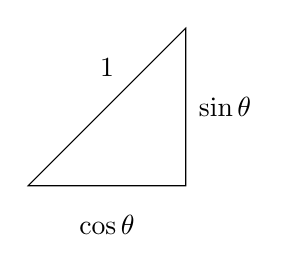
\begin{tikzpicture}[scale=0.5]
          \draw (0, 0) -- (4,0) -- (4, 4) -- cycle;
          \node at (2, -1) {$\cos \theta$};
          \node at (5, 2) {$\sin \theta$};
          \node at (2, 3) {1};
        \end{tikzpicture}
     \end{figure}
\end{columns}


\end{frame}
   
\begin{frame}[fragile, allowframebreaks]{절댓값과 유클리드 거리}
  \begin{description}
  \item[절댓값] 어떤 수와 0과의 수직선과의 거리, $|$를 사용해서 숫자의 앞 뒤를 감싸서 표현. $|3|=3, |-3| = 3$과 같이 표현됨
  \item[유클리드 거리] 좌표계 상의 두 점을 잇는 최단 거리의 선\\
    $ a$ 의 좌표 $(a_x, a_y)$ $b$의 좌표 $(b_x, b_y)$라고 할 때 이 두 점의 유클리드 거리는 다음과 같음. 
    \begin{equation*}
      \sqrt {\left(a_x - b_x \right)^2 + \left(a_y - b_y \right)^2}
    \end{equation*}
  \end{description}

\end{frame}
  
\begin{frame}[fragile,allowframebreaks]{수열}
  \begin{description}
  \item[수열] 여러 숫자가 줄지어 나열된 것을 표현함. 공학에서는 일정한 패턴을 갖는 수열을 주로 다룸
  \item[항] 수열을 구성하는 하나의 숫자\\ 
    \begin{equation*}
      a_1, a_2, a_3, a_4, \ldots, a_n 
    \end{equation*}
    $a_1$을 첫 항 또는 초항이라고 하고 $a_n$을 끝 항 또는 말항이라고 함
  \item[등차수열] 각 항의 차(공차, common difference)가 일정한 수열
  \item[등차수열의 일반항] 초항 $a$, 공차가 $d$일 때, 등차수열의 제 $n$항 $a_n$은 다음과 같이 정의한다. \\
    \begin{equation*}
      a_n =a + (n-1)d
    \end{equation*}
  \item[등차수열의 합] 초항이 $a$, 말항이 $l$, 항의 개수는 $n$, 초항에서 말항까지의 합이 $S$라고 할 때, 다음의 식이 성립함
    \begin{equation*}
      S = \frac{1}{2}n(a+l)
    \end{equation*}
  \item[등비수열] 인접하는 항의 비율이 일정한 수열, $1, 2, 4, 8, 16, 32, \ldots$ 일반적으로 등비수열은 $a, ar, ar^2, ar^3, \ldots, ar^n$과 같은 형태가 됨. 
  \item[공비] 등비수열에서 인접하는 항의 비율 $a_{n+1} = 2 \times a_n$
  \item[등비수열의 일반항] 초항이 $a$, 공비가 $r$일 때, 등비수열의 제 $n$항 $a_n$은 다음과 같이 정의함\\
    \begin{equation*}
      a_n = ar^{n-1}
    \end{equation*}
  \item[등비수열의 합] 초항이 $a$, 공비가 $r$, 초항에서 제 $n$항까지의 합이 $S_n$이라고 할 때 다음과 같은 식이 성림함
    \begin{eqnarray*}
      \text{if}~~ r\neq 1, S_n& = &\frac{a(1-r^n)}{1-r} = \frac{a(r^n-1)}{r-1} \\
      \text{if}~~ r =1, S_n &=& na
    \end{eqnarray*}
  \item[총합] $\sum$이라는 기호를 쓰고 각 항의 합을 뜻함\\
    \begin{eqnarray*}
      \sum_{k=1}^4 (3k + 1) & = & (3\times 1 + 1) +  (3 \times 2 + 1) \\&&+ (3 \times 3 + 1) + (3 \times 4 + 1) \\
                            & = & 4 + 7 + 10 + 13 \\
      & = & 34
    \end{eqnarray*}\\
    
  \item[기억할 공식] 다음 4 개의 식은 기억해두면 좋음\\[2em]
    \begin{tabular}[h]{l l}
      $\sum_{k=1}^n k = \frac{1}{2}n(n+1)$ & $\sum_{k=1}^n k^2 = \frac{1}{6}n(n+1)(2n+1)$ \\[2em]
      $\sum_{k=1}^n k^3 = \left(\frac{1}{2}n(n+1)\right)^2$ & $\sum_{k=1}^n c = nc$, $c$는 상수 \\[2em]
    \end{tabular}
  \item[총승의 성질] 다음과 같은 성질을 갖음\\
    \begin{eqnarray*}
      \sum_{k=1}^n (a_k + b_k) = \sum_{k=1}^n a_k + \sum_{k=1}^n b_k \\
      \sum_{k=1}^n pa_k = p\sum_{k=1}^n a_k, p = 상수
    \end{eqnarray*}
  \item[총승] $\prod$ 이라는 기호를 쓰고 각 항의 곱을 뜻함\\
    \begin{eqnarray*}
    Let~~ a_k &=& k-1 \\
      \prod_{k=1}^4 a_k &=& a_1 \times a_2 \times a_3 \times a_4 \\
      &=& 1 \times 3 \times 5\times 7 \\
      &=& 105
    \end{eqnarray*}
  \end{description}
\pagebreak
\begin{eqnarray*}
    y &=& 
    \left[
      \begin{array}{c c c c c }
         x_1  & x_2 & x_3 & \ldots & x_n
      \end{array}
    \right] \times
    \begin{bmatrix}
               w_{1} \\
               w_{2} \\
               w_{3} \\
               \vdots \\
               x_{n}
             \end{bmatrix} +b    \\[3em]
y & = &  x_1 \cdot w_1 + x_2 \cdot w_2 + \cdots + x_n\cdot w_n + b\\
&=& \sum _{k=1}^ n x_k w_k + b   
\end{eqnarray*}

\end{frame}
  
\begin{frame}[fragile,allowframebreaks]{집합과 원소}
\begin{description}
    \item[집합] set, 어떤 조건을 만족하는 것들을 중복되지 않도록 모두 모은 모둠. $\{$ 과 $\}$으로 원소를 감싸는 모양으로 표기
    \item[원소] element, 이 집합에 들어가는 각각의 것  
\end{description}

\begin{block}{표기 방법}
    \begin{itemize}
        \item $\{2, 4, 6, 8, 10\}$
        \item $\{x | x $ 조건 $\}$
    \end{itemize}
\end{block}

만약 어떤 원소 $x$가 $A$에 속한다면 $x \in A$ 그렇지 않다면 $x \notin A$

두 개의 집합 A, B가 있을 때 두 집합의 원소가 서로 완전히 일치하면 $A= B$이라고 표현

\begin{description}
    \item[부분집합] 집합 $B$의 모든 원소가 집합 $A$의 원소라면 집합 B는 A의 부분집합이라고 표현
    \item[교집합] intersection, 두 개의 집합이 있을 때 두 개의 집합에 모두 속하는 원소들의 집합, $A \cap B$
    \item[합집합] union, 두 개의 집합이 있을 때 적어도 한 집합에 속하는 원소들의 집합, $A \cup B$
    \item[공집합] 원소가 하나도 없는 집합. $\phi$로 표현하고 $\phi$는 모든 집합의 부분집합임. 어떤 집합 $A$가 있을 때 $\phi \subset A$라고 할 수 있음  
\end{description}
\pagebreak

\colorlet{circle edge}{blue!50}
\colorlet{circle area}{blue!20}
\tikzset{filled/.style={fill=circle area, draw=circle edge, thick},
    outline/.style={draw=circle edge, thick}}
\def\firstcircle{(0,0) circle (1.cm)}
\def\secondcircle{(0:1.5cm) circle (1.cm)}

\begin{columns}
    \column{0.45\textwidth}
    \begin{tikzpicture}
        \begin{scope}
            \clip \firstcircle;
            \fill[filled] \secondcircle;
        \end{scope}
        \draw[outline] \firstcircle node {$A$};
        \draw[outline] \secondcircle node {$B$};
        \node[anchor=south] at (current bounding box.north) {$A \cap B$};
    \end{tikzpicture}
    
    %Set A or B but not (A and B) also known a A xor B
    \begin{tikzpicture}
        \draw[filled, even odd rule] \firstcircle node {$A$}
        \secondcircle node{$B$};
        \node[anchor=south] at (current bounding box.north) {$\overline{A \cap B}$};
    \end{tikzpicture}
    
    \column{0.45\textwidth}\vspace{-7.4em}

% Set A or B
\begin{tikzpicture}
    \draw[filled] \firstcircle node {$A$}
                  \secondcircle node {$B$};
    \node[anchor=south] at (current bounding box.north) {$A \cup B$};
\end{tikzpicture}

% Set A but not B
\begin{tikzpicture}
    \begin{scope}
        \clip \firstcircle;
        \draw[filled, even odd rule] \firstcircle node {$A$}
                                     \secondcircle;
    \end{scope}
    \draw[outline] \firstcircle
                   \secondcircle node {$B$};
    \node[anchor=south] at (current bounding box.north) {$A - B$};
\end{tikzpicture}

% Set B but not A
\begin{tikzpicture}
    \begin{scope}
        \clip \secondcircle;
        \draw[filled, even odd rule] \firstcircle
                                     \secondcircle node {$B$};
    \end{scope}
    \draw[outline] \firstcircle node {$A$}
                   \secondcircle;
    \node[anchor=south] at (current bounding box.north) {$B - A$};
\end{tikzpicture}

\end{columns}


\end{frame}
   
\section{미분}
\begin{frame}[fragile]{극한}
\begin{description}
    \item[극한] 수열이나 함숫값이 어떤 특정 값에 한없이 가까워지는 것을 의미
    \item[수렴] convergent, $x$의 값을 어떤 값 $a$에 최대한 가깝게 만들 때, 함수 $f(x)$의 어떤 값 $a$에 최대한 가까워지는 모양
    \item[극한값] limit, limiting value. 수렴하려는 값을 표현. $a$ 는 함수 $f(x)$에서 $x \rightarrow a$일 때의 극한값이라고 표현
    \begin{eqnarray*}
        \lim _{x \rightarrow a} f(x) = \alpha,~~~~~~~~
        f(x) \rightarrow \alpha (x \rightarrow a)
    \end{eqnarray*}  
\end{description}

\begin{columns}
    \column{0.25\textwidth}\vspace{-11em}
    \[f(x) = \frac{x^2-1}{x-1}\]
    \[\lim _{x \rightarrow 1} \frac{x^2-1}{x-1}\]
    \[=\lim _{x \rightarrow 1} \frac{(x-1)(x+1)}{x-1}\]
    \[=\lim _{x \rightarrow 1} (x+1) =2\]
    \column{0.35\textwidth}
    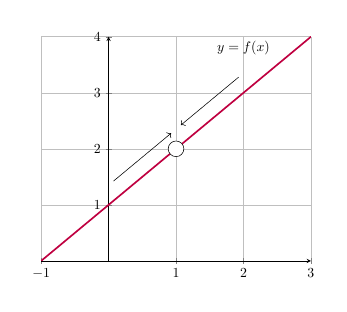
\begin{tikzpicture}[scale = 0.5]
        \begin{axis}[axis lines=middle, grid]
            \addplot[smooth,domain=-1:3,purple,very thick] {(x*x-1)/(x-1)}; 
            \node[circle,fill=white, draw,inner sep=4pt] at (axis cs:1,2) {};
            \node at (axis cs:2,3.8) {$y=f(x)$};
            \begin{scope}[yshift=0.5cm]
                \node[fill=none] (a) at (axis cs:0,1){};\node[fill=none] (b) at (axis cs:1,2){};
                \node[fill=none] (c) at (axis cs:2,3){};
                \draw[->] (a) -- (b);
                \draw[->] (c) -- (b);
            \end{scope}
        \end{axis}
    \end{tikzpicture}
\column{0.40\textwidth}\vspace{-8em}

$f(x)$는 $x=1$일 때 분모가 $0$이 되기 때문에 $y$를 정의할 수 없음. $x\neq1$일 때는 정의 가능
\end{columns}
\end{frame}

\begin{frame}[fragile,allowframebreaks]{미분의 기초}
    \begin{block}{예제}
        강남역에서 인천공항까지 72.56km의 거리를 자동차로 이동하는데 1시간 반이 걸렸다. 이때의 이동 평균 속도를 구하라.
\begin{eqnarray*}
    \text{평균 속도} v &=& \frac{72.56km}{1.5h} \approx 48.37km/h \\
        \text{순간 속도 } v &=& \lim _{\Delta t \rightarrow 0} \frac{\Delta x}{ \Delta t}\\
        &=&\lim _{\delta t \rightarrow 0} \frac{x(x+\delta x)-x(t)}{ \Delta t}\\
        \text{미분 표기법} && \frac{dx(t)}{dt}
\end{eqnarray*}
    \end{block}

\pagebreak
\begin{columns}
    \column{0.45\textwidth} \vspace{-2em}
    \begin{block}{미분 풀이}
        \begin{eqnarray*}
        y &=& f(x)\\
        y &=& \alpha x + \beta\\
        \\
        \text{식 1: } f(a) &=& \alpha a + \beta \\
        \text{식 2: }f(b) &=& \alpha b + \beta \\ \\
        f(b) - f(a) &=& \alpha (b -a)\\
        \text{식 3: }\alpha &=& \frac{f(b)-f(a)}{b-a} \\ \\
        \beta &=& f(a) -\alpha a \\
        &=& f(a) - \frac{f(b)-f(a)}{b-a} a
        \end{eqnarray*}
        \end{block}
    \column{0.45\textwidth}

    \begin{itemize}
        \item 식 3: 기울기 $\alpha$ -- 두 점 사이에서 평균적으로 변화한 정도. 평균변화율
        \item 이해: 함수 $f(x)$ 위의 점 $(a, f(x))$ 에서 순간적으로 변화는 정도 (기울기)\\$alpha = \frac{\text{d}f(x)}{\text{d}x}$
        \item 어떤 함수의 특정한 지점의 기울기를 구하는 것을 미분한다고 표현
    \end{itemize}

\end{columns}
\pagebreak
\begin{columns}
    \column{0.45\textwidth} \vspace{-2em}
    \begin{block}{미분한다}
        \begin{eqnarray*}
            \frac{\text{d}f(a)}{\text{d}a} &=& \lim _{\Delta x \rightarrow 0} \frac{\Delta f(a)}{\Delta x} \\
            &=& \lim _{\Delta h \rightarrow 0} \frac{f(a+h)-f(a)}{(a+h)-a} \\
            &=&  \lim _{\Delta h \rightarrow 0} \frac{f(a+h)-f(a)}{h}
        \end{eqnarray*}
            
    \end{block}
    \begin{itemize}
        \item \textbf{접선}: 함수 $f(x)$위의 한 점 $a$을 지나는 직선
        \item \textbf{미분계수}: 평균변화율의 극한 값인 $\alpha$는 $x=a$일 때의 미분계수라고 함
    \end{itemize}
    \column{0.45\textwidth}
    \begin{itemize}
        \item 상수 $a$는 변수 $x$가 가질 수 있는 수 많은 값들 중 하나임. 
        \item 상수 $a$에 어떤 $x$를 대입하더라도 $\frac{\text{d}f(a)}{\text{d}x}x$의 값은 결정되므로 $\frac{\text{d}f(a)}{\text{d}x}x$는 $x$에 대한 일종의 함수
        \item $\frac{\text{d}f(x)}{\text{d}x}x$라 쓰고 도함수(derivative)라고 부름.
    
    \end{itemize}
    \begin{eqnarray*}
        y &=& \frac{\text{d}f(a)}{\text{d}x}x + \left( f(a)- \frac{\text{d}f(a)}{a} \right)\\
        &=& \frac{\text{d}}{f(a)}(x-a)+f(a)
    \end{eqnarray*}
\end{columns}
\end{frame}


\begin{frame}[fragile,allowframebreaks]{상미분과 편미분}
    \begin{block}{상미분}
        Ordinary derivative, 변수가 하나만 있는 함수의 미분 
    \end{block}
\begin{enumerate}
    \item $y = x^r$일 때 $\frac{\text{d}f(x)}{x}=rx^{r-1} $, 이 때 $r$은 임의의 실수
    \item $\frac{\text{d}}{x}\left( f(x)+g(x) \right) = \frac{\text{d}f(\text{d}x)}{\text{d}x}+ \frac{\text{d}g(x)}{\text{d}x}$
    \item $\frac{\text{d}}{\text{d}x}\left( kf(x)\right) = k\frac{\text{d}f(x)}{x}$
\end{enumerate}
\begin{block}{전미분}
    Total derivative, 변수가 두 개  이상이 있는 함수의 미분 
\end{block}
\begin{eqnarray*}
    z &=&f(x, y)\\
    &=& 3x^2 + 2xy + 2y^2\\
    \Delta z &=& f(x+\Delta x, y  + \Delta y) - f(x, y)\\
    &=& 3(x+\Delta x)^2 + 2(x+\Delta x)(y+\Delta y) 2(x+\Delta y)^2 - (3x^2 + 2xy + 2y^2)\\
    &=& (6x + 2y)\Delta x + (2x+4y)\Delta y + 3 \Delta x^2 + 2 \Delta x \Delta y + 2 \Delta y^2
\end{eqnarray*}



\begin{block}{편미분}
    partial derivative, 변수가 두 개  이상일 때 하나의 변수 외에는 고정을 시킨 함수의 미분 \\
    $\Delta y = 0$일 때 $\Delta x \rightarrow 0$로 변화시키는 것
\end{block}
\begin{eqnarray*}
    \frac{\delta f(x, y)}{\delta x} &=& \lim _{\Delta x \rightarrow 0} \frac{\Delta z}{\Delta x} \\
    &=& \lim _{\Delta x \rightarrow 0} 6x + 2y + 3\Delta x \\
    &=& 6x + 2y
\end{eqnarray*}

\begin{equation*}
    \frac{\delta f(x, y)}{\delta y} = 2x + 4y
\end{equation*}

편미분을 간단하게 다음과 같이 표현할 수 있음\\ $\frac{\delta f(x, y)}{\delta x}$는 $f_x(x, y)$, $\frac{\delta f(x, y)}{\delta t}$는 $f_y(x, y)$

\end{frame}


\begin{frame}[fragile,allowframebreaks]{그래프 그리기}
    \begin{tikzpicture}[scale=0.8]
        \draw [->] (-1,0) -- (11,0) node [right] {$x$};
        \draw [->] (0,-1) -- (0,6) node [above] {$y$};
        \node at (0,0) [below left] {$0$};
        \draw  plot[smooth, tension=.7] coordinates{(1.5,-0.5) (3,3) (5,1.5)  (7.5,4) (10,-1)};
        \node at (1.75,-0.25) {$a$};
        \node at (9.5,-0.25) {$b$};
        \draw[dashed] (3.2,3.05) -- (3.2,0);
        \draw[dashed] (4.9,1.5) -- (4.9,0);
        \draw[dashed] (7.3,4.05) -- (7.3,0);
        \node at (3.2,-0.25) {$c_{1}$};
        \node at (4.9,-0.25) {$c_{2}$};
        \node at (7.3,-0.25) {$c_{3}$};
        \draw (2.5,3.05) -- (4,3.05);
        \draw (4,1.5) -- (6,1.5);
        \draw (6.5,4.05) -- (8.25,4.05);
        \node at (3.2,3.5) {$f'(c_{1})=0$};
        \node at (4.9,2.2) {$f'(c_{2})=0$};
        \node at (7.3,4.5) {$f'(c_{3})=0$};
        \node at (9.5,2.5) {$y=f(x)$};
   \end{tikzpicture}

\pagebreak
\begin{tabular}{|c | c | c | c |} \hline
    $\frac{\text{d}x}{\text{d}t}$ &$\frac{\text{d}^2x}{\text{d}t^2}$ & 화살표 & 의미 \\ \hline \hline 

    0 & NA & 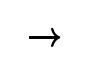
\begin{tikzpicture}[scale=0.2]
        \path[->, line width = 0.8pt] (0,0) edge[right] (2,0);
      \end{tikzpicture} & $x$는 일정 $\left(\frac{\text{d}x}{\text{d}t} =0\right)$ \\ \hline
    
    $+$ & $+$ & 
\begin{tikzpicture}[scale=0.2]
        \path[->, line width = 0.8pt] (0,0) edge[bend right] (2,2);
      \end{tikzpicture} & $x$는 증가 $\left(\frac{\text{d}x}{\text{d}t} > 0\right)$ 하고, 증가율이 증가 $\left(\frac{\text{d}^2x}{\text{d}t^2} > 0\right)$ \\ \hline
    
    $+$ & $0$ & 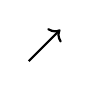
\begin{tikzpicture}[scale=0.2]
        \path[->, line width = 0.8pt] (0,0) edge[right] (2,2);
      \end{tikzpicture} & $x$는 증가 $\left(\frac{\text{d}x}{\text{d}t} > 0\right)$ 하고, 증가율이 일정 $\left(\frac{\text{d}^2x}{\text{d}t^2} = 0\right)$ \\ \hline

    $+$ & $-$ & 
\begin{tikzpicture}[scale=0.2]
        \path[->, line width = 0.8pt] (0,0) edge[bend left] (2,2);
      \end{tikzpicture} & $x$는 증가 $\left(\frac{\text{d}x}{\text{d}t} > 0\right)$ 하고, 증가율이 감소 $\left(\frac{\text{d}^2x}{\text{d}t^2} < 0\right)$ \\ \hline \hline

    $-$ & $+$ & 
\begin{tikzpicture}[scale=0.2]
        \path[->, line width = 0.8pt] (0,0) edge[bend right] (2,-2);
      \end{tikzpicture} & $x$는 감소 $\left(\frac{\text{d}x}{\text{d}t} > 0\right)$ 하고, 감소율이 감소 $\left(-\frac{\text{d}^2x}{\text{d}t^2} < 0\right)$ \\ \hline
    
    $-$ & $0$ & 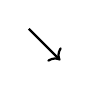
\begin{tikzpicture}[scale=0.2]
        \path[->, line width = 0.8pt] (0,0) edge[right] (2,-2);
      \end{tikzpicture} & $x$는 감소 $\left(\frac{\text{d}x}{\text{d}t} < 0\right)$ 하고, 감소율이 일정 $\left(-\frac{\text{d}^2x}{\text{d}t^2} = 0\right)$ \\ \hline

    $-$ & $-$ & 
\begin{tikzpicture}[scale=0.2]
        \path[->, line width = 0.8pt] (0,0) edge[bend left] (2,-2);
      \end{tikzpicture} & $x$는 감소 $\left(\frac{\text{d}x}{\text{d}t} < 0\right)$ 하고, 감소율이 증가 $\left(-\frac{\text{d}^2x}{\text{d}t^2} > 0\right)$ \\ \hline

\end{tabular}

\textbf{변곡점:}
    그래프 상에서 곡선의 방향이 바뀌는 지점을 말함. 변곡점에서 2계미분을 하면 값이 0이 됨. 값의 앞과 뒤 점에서의 부호가 반전됨.\\
\textbf{극값, 극대 또는 극소:}
    변곡점 중 최대 또는 최소 값을 갖는 점을 극대 또는 극소라 하고 통틀어서 극값이라고 함.    

\end{frame}

\begin{frame}[fragile]{함수의 최댓값과 최소값}
\begin{description}
    \item[최댓값과 최솟값] 극점 또는 함수가 정의된 구간 양끝단에서 나옴
\end{description}

\begin{center}
    \begin{tabular}{|c || c | c | c | c | c| } \hline
        x & -3 & $\cdots$ & 1 &$\cdots$ & 10 \\ \hline \hline
        $\frac{\text{d}f(x)}{\text{d}x}$ & - & - & 0 & + & + \\ \hline
        $\frac{\text{d}^2f(x)}{\text{d}x^2}$ & + & + & +& + & + \\ \hline
        $f(x)$ & 20 & 
\begin{tikzpicture}[scale=0.2]
            \path[->, line width = 0.8pt] (0,0) edge[bend right] (2,-2);
          \end{tikzpicture} & 4 & 
\begin{tikzpicture}[scale=0.2]
            \path[->, line width = 0.8pt] (0,0) edge[bend right] (2,2);
          \end{tikzpicture} & 85 \\ \hline
    \end{tabular}    
\end{center}
\end{frame}

\begin{frame}[fragile,allowframebreaks]{초등함수와 합성함수의 미분, 그리고 곱의 법칙}

    \begin{description}
        \item[초등함수] $x^r$ (멱함수), $a^x$ (지수함수), $\log_c x$ (로그함수), 삼각함수 등을 통틀어 초등함수(elementary function)라 부름
    \end{description}

    초등함수의 미분 공식 \vspace{-2em}
    \begin{table}
    \begin{tabular}{|c | c| c | c|}\hline
        \multicolumn{3}{|c|}{원래 함수} & 원래 함수를 $x$로 미분한 것 \\ \hline
        \multicolumn{2}{|c|}{역함수} & $x^r$ & $rx^{r-1}$ \\ \hline
        \multicolumn{2}{|c|}{\multirow{2}{*}{지수함수}} & $e^x, \exp(x)$ & $e^x, \exp(x)$ \\ \cline{3-4}
        \multicolumn{2}{|c|}{}& $a^x$ & $a^x\log _e ^a$ \\ \hline
        \multicolumn{2}{|c|}{로그함수} & $\log _e x ~~~(x>0)$ & $\frac{1}{x}$ \\ \hline
        \multirow{3}{*}{삼각함수} &  사인함수 & $\sin (x)$ &  $\cos (x)$ \\ \cline{2-4}
        & 코사인함수 & $\cos (x)$ &  $-\sin (x)$ \\ \cline{2-4}
        & 탄젠트함수 & $\tan (x)$ &  $\frac{1}{\cos^ (x)}$ \\ \hline
        
        
    \end{tabular}
    \end{table}
\pagebreak

\begin{columns}
    \column{0.35\textwidth}

사인과 코사인의 관계
\begin{tikzpicture}% 
    [->, thick, scale = 0.3]
    \node (1) at (3, 3) {$\sin (x)$};
    \node (2) at (-3, 3) {$\cos(x)$};
    \node (3) at (-3, -3) {$-\sin(x)$};
    \node (4) at (3, -3) {$-\cos(x)$};

    \draw (1) [out=135, in =45] to node [midway, above] {미분} (2) ;
    \draw (2) [out=225, in =135] to node [midway, above, rotate=90] {미분} (3);
    \draw (3) [out=315, in =225] to node [midway, below] {미분} (4);
    \draw (4) [out=45, in =315] to node [midway, below, rotate=90] {미분} (1);
\end{tikzpicture}

\column{0.65\textwidth}
\textbf{공식}
\begin{itemize}
    \item \textbf{합성함수 미분(변수 한 개)}: $y=f(x)$ \[\frac{\text{d}y}{\text{d}x} = \frac{\text{d}y}{\text{d}u}\cdot \frac{\text{d}u}{\text{d}x}  \]
    \item \textbf{합성함수 미분(변수 여러 개)}: 연쇄 법칙(chain rule)이 적용됨 $z=f(x,y)$ \[\frac{\text{d}z}{\text{d}x} = \frac{\text{d}z}{\text{d}u}\cdot \frac{\text{d}u}{\text{d}x} + \frac{\text{d}z}{\text{d}v}\cdot \frac{\text{d}v}{\text{d}x} \]
    \item \textbf{곱의 법칙}  \[\frac{\text{d}}{\text{d}x}\left(f(x)g(x)\right) = \frac{\text{d}(x)}{\text{d}x}g(x) + f(x)\frac{\text{d}g(x)}{\text{d}x} \]
\end{itemize}
\end{columns}

\pagebreak
\begin{block}{예: $f(x)=(3x-4)^{50}$ 의 미분} 
    $u=3x-4$ 라고 하자. 이 때 다음과 같이 표현할 수 있음.
    \[\frac{\text{d}f(x)}{\text{d}x}=\frac{\text{d}f(x)}{\text{d}u} \cdot \frac{\text{d}u}{\text{d}x} \]
    계산하면 다음과 같음.
    \begin{eqnarray*}
        \frac{\text{d}f(x)}{\text{d}x}&=& \frac{\text{d}u^{50}}{\text{d}u} \cdot \frac{\text{d}(3x-4)}{\text{d}x}\\
        &=& 50u^{49} \cdot 3\\
        &=& 150 (3x-4 )^{49}   
    \end{eqnarray*}
\end{block}

\end{frame}

\begin{frame}[fragile,allowframebreaks]{특수 함수의 미분}
        \text{시그모이드 함수}
        \begin{eqnarray*}
        \varsigma_a(x) &=&
         \frac{1}{1+\exp(-ax)}\\[0.5em]
        \end{eqnarray*}

         \text{미분}
         \begin{eqnarray*}
        \frac{\text{d}\varsigma_a(x)}{\text{d}x} &=& \frac{a \cdot \exp(-ax)}{\left(1 + \exp(-ax)\right)^2} \\
        &=& a\varsigma_n(x)\left(1 - \varsigma_a (x)\right)
        \end{eqnarray*}
    
        \pagebreak

    시그모이드 함수의 2차 미분
        \begin{eqnarray*}
        \frac{\text{d}^2\varsigma_a(x)}{\text{d}x^2} &=& \frac{\text{d}\left(a\varsigma_a(x) \left(1 - \varsigma_a(x)\right))\right)}{\text{d}x}\\
        &=&a\frac{\text{d}\varsigma_a(x)}{\text{d}x}\left(1-\varsigma_a(x)\right) + a\varsigma_a(x) \frac{\text{d}\left(1-\varsigma_a(x)\right)}{\text{d}x}\\
        &=&a\frac{\text{d}\varsigma_a(x)}{\text{d}x}\left(\varsigma_a(x)\right) + a\varsigma_a(x) \frac{\text{d}\left(1-\varsigma_a(x)\right)}{\text{d}x}\\
        &=&a\frac{\text{d}\varsigma_a(x)}{\text{d}x}\left(1-2\varsigma_a(x)\right) \\
        &=& a^2\varsigma_a(x)\left(1-\varsigma_a(x)\right)\left(1-2\varsigma_a(x)\right)
    \end{eqnarray*}

    \pagebreak

    \begin{columns}
        \column{0.5 \textwidth}
    표준 시그모이드 함수 $(a = 1)$
    \begin{tikzpicture}[scale=0.7]
        \begin{axis}[ymax=1, xmin=-20, xmax=20,domain=-20:20,axis lines=middle]
        \addplot[smooth,purple,very thick] {1/(1+exp(-x))};
        \node at (250, 50) {0.5};
        \end{axis}
    \end{tikzpicture}

    \column{0.5 \textwidth}
    표준 시그모이드 함수의 미분 \\
    \begin{tikzpicture}[ scale=0.7]
        \begin{axis}[ymax=1, xmin=-10, xmax=10,axis lines=middle]
        \addplot[smooth,purple,very thick] {1/(1+exp(-x))*(1- 1/(1+exp(-x)))};
        \node at (120, 250) {0.25};
        \end{axis}
    \end{tikzpicture}
    \end{columns}

    \pagebreak
    
    \begin{block}{ReLU (Rectified Linear Unit) 함수}

        \begin{eqnarray*}
            \varphi (x) = \max (0, x ) = \begin{cases}
                x & (x > 0) \\
                0 & (x \leq 0)
            \end{cases} \\
            \varphi'(x) = \begin{cases}
                1 & (x> 0)\\
                0 & (x \leq 0)
            \end{cases}
        \end{eqnarray*}
        
    \end{block}

    \begin{columns}
        \column{0.5\textwidth}
        \textbf{ReLU 함수 $\varphi(x)$의 그래프 }
        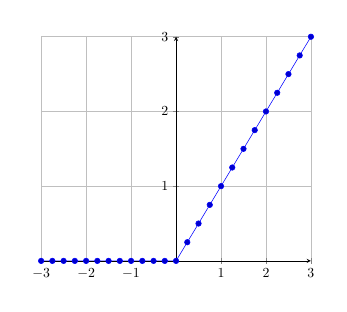
\begin{tikzpicture} [scale = 0.5]
            \begin{axis}[axis lines=middle,grid,
                domain=-3:3,
            ]
                \addplot {
                    ifthenelse(
                        x>0,        % if
                        x,        % then
                        0           % else
                    )
                };
            \end{axis}
        \end{tikzpicture}
        \column{0.5\textwidth}
        \textbf{ReLU 함수의 미분 $\varphi'(x)$ 그래프 }
        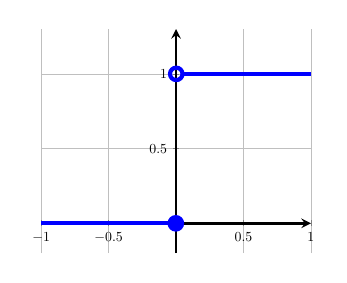
\begin{tikzpicture} [scale = 0.5]
            \begin{axis}[ymax=1.3, ymin= -0.2, xmin= -1, xmax= 1, axis lines=middle,grid,
             line width =2pt
            ]
            \addplot[line width = 3pt, blue,arrows=-*,samples at={-1.1,0.06}] {0};
            \addplot[line width = 3pt, blue,arrows=o-,mark options={fill=white}, samples at={-0.06,1.1}] {1};
            \end{axis}
        \end{tikzpicture}
    \end{columns}
\end{frame}
    

\section{선형대수}
\begin{frame}[fragile]{벡터}

    벡터를 표현하는 세 가지 방법
    \begin{itemize}
        \item $\mathbf{a}$ 출판물의 활자에 자주 사용됨
        \item $\vec{a}$ 벡터 표기할 때 자주 사용됨
        \item $\mathbb{A}$ 실수, 자연수 등을 표현하는데 사용되기 때문에 잘 안 쓰임
    \end{itemize}

    \let\oldhat\hat
    \renewcommand{\vec}[1]{\mathbf{#1}}
    \renewcommand{\hat}[1]{\oldhat{\mathbf{#1}}}

    \begin{columns}
        \column{0.45\textwidth}
        행벡터: 성분을 나열한 방식이 가로인 경우
\[\vec{a} = \begin{pmatrix}
    a_1 & a_2 & a_3 & \ldots & a_n 
\end{pmatrix}  \]

\column{0.45\textwidth}
열벡터: 성분을 나열한 방식이 세로인 경우
\[\vec{b} = \begin{pmatrix}
b_1 \\ 
b_2 \\ 
b_3 \\ 
\ldots \\ 
b_n 
\end{pmatrix}  \]

\end{columns}
    
\end{frame}

\begin{frame}[fragile]{덧셈과 뺄셈, 그리고 스칼라배}
    차원이 같은 경우만 덧셈, 뺄셈이 가능함\\[3em]
\begin{columns}
    \column{0.5\textwidth}
\textbf{벡터의 덧셈}
    \[\begin{pmatrix}
        1 \\
        2\\
        3
    \end{pmatrix} + \begin{pmatrix}
        4\\
        5\\
        6
    \end{pmatrix} = \begin{pmatrix}
        1+4 \\
        2+5 \\
        3+6 
    \end{pmatrix} = \begin{pmatrix}
        5 \\
        7 \\
        9 
    \end{pmatrix}\]

    \column{0.5\textwidth}
    \textbf{벡터의 뺄셈}
    \[\begin{pmatrix}
        1 \\
        2\\
        3
    \end{pmatrix} + \begin{pmatrix}
        4\\
        5\\
        6
    \end{pmatrix} = \begin{pmatrix}
        1-4 \\
        2-5 \\
        3-6 
    \end{pmatrix} = \begin{pmatrix}
        -3 \\
        -3 \\
        -3 
    \end{pmatrix}\]

    
\end{columns}
\begin{center}
    \textbf{벡터의 스칼라 배}    
\end{center}
    \[
        2 \cdot \begin{pmatrix}
        1 \\
        2\\
        3
    \end{pmatrix} = \begin{pmatrix}
        2\times1 \\
        2\times2 \\
        2\times3 
    \end{pmatrix} = \begin{pmatrix}
        2 \\
        4 \\
        6 
    \end{pmatrix}\]

\end{frame}

\begin{frame}[fragile,allowframebreaks]{유향성분}

\begin{columns}
    \column{0.6\textwidth}
    \begin{description}
        \item[유향성분] $\vec{a} = (4, 3)$은 오른쪽으로 4, 위쪽으로 3 움직이는 것과 같은 의미임. 이때 원점에서 특정 점 $(4,3)$을 잇는 최단 방향과 그 거리를 나타내는 화살표를 뜻함 
    \end{description}
    \begin{center}
    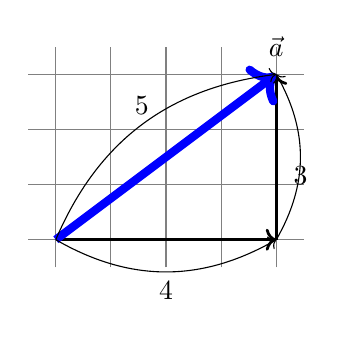
\begin{tikzpicture}% 
        [scale = 0.7]
        \draw[step=1.0,gray,thin] (-0.5,-0.5) grid (4.5,3.5);
        \node  at (4, 3.5) {$\vec{a}$};
    
        \draw [->,line width = 1pt] (0,0) to (4,0);
        \draw [->,line width = 1pt] (4,0) to (4,3);
        \draw [->,blue, line width = 3pt] (0,0) to (4,3);
        
        \draw [->] (0,0) [bend right] to node [midway, below] {4} (4,0) ;
        \draw [->] (4,0) [bend right] to node [midway, below ] {3} (4,3);
        \draw [->] (0,0) [bend left] to node [midway, above] {5} (4,3);
    \end{tikzpicture}
\end{center}
    \column{0.4\textwidth}

$\vec{a} = (1, 2), \vec{b} = (3, 1)$ 일 때 \[\vec{a} + \vec{b} = (4,3) \]
\begin{center}
    
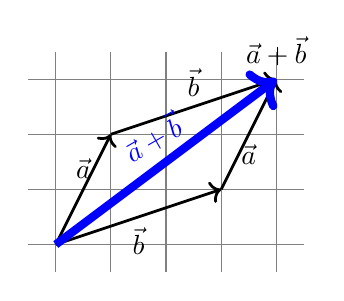
\begin{tikzpicture}% 
    [scale = 0.7]
    \draw[step=1.0,gray,thin] (-0.5,-0.5) grid (4.5,3.5);
    \node  at (4, 3.5) {$\vec{a}+\vec{b}$};

    \draw [->,line width = 1pt] (0,0) --   (1,2) node[midway, above] {$\vec{a}$};
    \draw [->,line width = 1pt] (1,2) -- (4,3) node [midway, above] {$\vec{b}$};
    
    \draw [->,line width = 1pt] (0,0) -- (3,1) node [midway, below] {$\vec{b}$};
    \draw [->,line width = 1pt] (3,1) -- (4,3) node [midway, below] {$\vec{a}$};
    
    \draw [->,blue, line width = 3pt] (0,0) -- (4,3) node [midway, above, rotate= 30] {$\vec{a}+ \vec{b}$};
        
\end{tikzpicture}\end{center}
\end{columns}

\pagebreak

\begin{columns}
\column{0.4\textwidth}    
$\vec{a} = (1, 2), \vec{b} = (3, 1)$ 일 때 
\begin{itemize}
    \item $-\vec{a} $
    \item $\vec{a} - \vec{b} $
    \item $- \vec{b} $
\end{itemize}

\column{0.6\textwidth}    
    \begin{center}
    
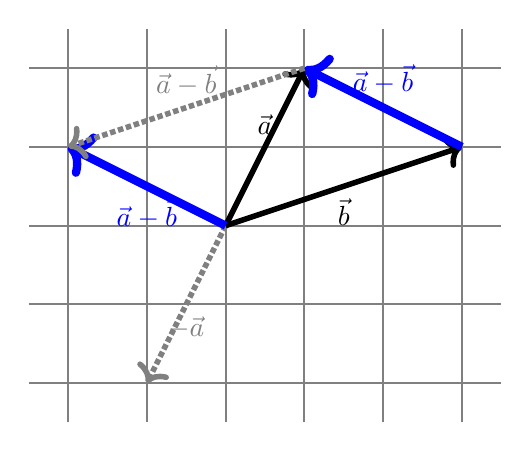
\begin{tikzpicture}% 
    [scale = 1]
    \draw[step=1.0,gray,thick] (-2.5,-2.5) grid (3.5,2.5);
    
    \draw [->,line width = 2pt] (0,0) --   (1,2) node[midway, above] {$\vec{a}$};
    \draw [->,gray, densely dotted, line width = 2pt] (0,0) --   (-1,-2) node[midway, below] {$-\vec{a}$};

    \draw [->,line width = 2pt] (0,0) -- (3,1) node [midway, below] {$\vec{b}$};
    
    \draw [->,blue, line width = 3pt] (3,1) -- (1,2) node [midway, above] {$\vec{a}-\vec{b}$};
    \draw [->,blue, line width = 3pt] (0,0) -- (-2,1) node [midway, below] {$\vec{a}-\vec{b}$};
    

    \draw [->,densely dotted, gray, line width = 2pt] (1,2) -- (-2,1) node [midway, above] {$\vec{a} - \vec{b}$};
        
\end{tikzpicture}\end{center}
\end{columns}
    
\end{frame}



\begin{frame}[fragile,allowframebreaks]{내적}
\begin{description}
    \item[내적] 벡터에서 서로 대응하는 성분끼리 곱한 다음 그것들을 모두 더한 값. $\vec{a} \cdot \vec{b}$ 로 표현되기도 하고 $\langle \vec{a}, \vec{b} \rangle$ 로 표기하기도 함 \\
    벡터의 내적은 벡터가 아니라 스칼라가 됨
\end{description}
\[\vec{a} = \begin{pmatrix}
    a_1 \\
    a_2 \\
    \vdots \\
    a_n
\end{pmatrix} , \vec{b} = \begin{pmatrix}
    b_1 \\
    b_2 \\
    \vdots \\
    b_n
\end{pmatrix} \text{일 때} \]
\begin{eqnarray*}
    \langle \vec{a}, \vec{b} \rangle &=& a_1 b_1 + a_2 b_2 + \ldots + a_n b_n\\ 
    &=& \sum _{i=1} ^n = a_i b_i
\end{eqnarray*}

내적의 다른 말: 점곱 (dot product), 스칼라곱 (scalar product), 영사곱 (projection product) 

외적의 다른 말: 교차곱 (cross product), 벡터곱 (vector product), 텐서곱 (tensor product)

\pagebreak

\begin{block}{기하학적 특징}
    벡터 $\vec{a}$와 $\vec{b}$가 이루는 각이  $\theta$일 때, $\langle \vec,{a}, \vec{b} \rangle$는 다음과 같이 정의할 수 있음
    \[ \langle \vec{a}, \vec{b} \rangle = \|\vec{a}\| \|\vec{b} \| \cos \theta \]
    이 때 $\theta$ 는 $\vec{a}$와 $\vec{b}$의 시작점을 일치시킬 때 생기는 사이각을 말함. $\|\vec{a}\|$는 벡터의 길이 또는 유클리드 거리를 의미함.
\end{block}

\begin{columns}
    \column{0.3\textwidth}
    
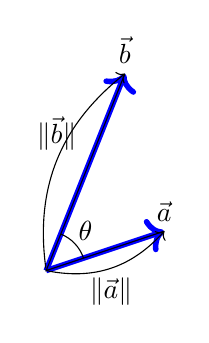
\begin{tikzpicture}[scale =0.5]
    \draw[->, line width = 2pt, blue] (0,0) -- (2, 5) ;
    \draw [->] (0,0)  [bend left] to node [midway, above] {$\|\vec{b}\|$} (2,5);
    
    \draw[->, line width = 2pt, blue] (0,0) -- (3, 1) ;
    \draw [->] (0,0)  [bend right] to node [midway, below] {$\|\vec{a}\|$} (3,1);

    \draw (3,1) coordinate (x) -- (0,0) coordinate (y) -- (2,5) coordinate (z) pic [draw] {angle = x--y--z} ;
    
    \node at (1,1) {$\theta$};
    \node [above] at (2,5) {$\vec{b}$};
    \node [above] at (3,1) {$\vec{a}$};
\end{tikzpicture}
\column{0.7\textwidth}

\begin{eqnarray*}
    \langle \vec{a}, \vec{b} \rangle = 2 \times 1 + 1\times 3 
    = 2 + 3 = 5    \\[1em]
    \| \vec{a} \| = \sqrt{2^2 + 1^2} = \sqrt{5}, \| \vec{b} \| = \sqrt{1^2 + 3^2} = \sqrt{10}\\ 
    \langle \vec,{a}, \vec{b} \rangle  = \|\vec{a}\| \|\vec{b} \| \cos 45^{\circ} = \sqrt{5} \times \sqrt{10} \times \frac{\sqrt{2}}{2} = 5
\end{eqnarray*}
\end{columns}
\end{frame}



\begin{frame}[fragile]{직교 조건}
    두 개의 벡터가 직교한다(수직으로 만난다)는 것은 두 벡터가 이루는 각이 $90^{\circ}$라는 뜻임
    \[ \langle \vec{a}, \vec{b} \rangle = \|\vec{a}\| \|\vec{b} \| \cos 90^{\circ} \]

    이 때 $\cos 90^{\circ}=0$이기 때문에 두 벡터의 내적은 0이 됨.
\end{frame}


\begin{frame}[fragile]{법선벡터}
    예를 들어 구 표면 위의 하나의 점에 접하는 접선을 구했을 때, 접선이 존재하는 평면. 이를 접평면 (tangent plane)이라고 하고, 접평면과 구와 접하는 점을 접점이라고 함

    접선과 직교하는 벡터를 통해 접평면을 다룰 수 있는 개념으로 법선벡터을 사용함
\end{frame}




\begin{frame}[fragile]{벡터의 노름 (norm)}
\begin{description}
    \item[노름 (norm)] 벡터의 시작점에서 도착점까지 도달하기 위한 $x$, $y$에서 이동한 거리. 예: $\vec{a} = (4,3)$ 일 때,  오른쪽으로 4, 위로 3 이동하여 총 7만큼 이동함. 이렇게 구한 움직인 거리를 $L1 norm$이라고 함. 또는 맨해튼 거리라고도 함.
\end{description}

\begin{block}{$\vec{a}$에 대한 $L1$ norm}
    \[\|a\|_1 = |a_1| +|a_2| + \cdots +|a_n| = \sum_{i=1}^n |a_i|     \]
    
\end{block}

\begin{block}{$\vec{a}$에 대한 $L2$ norm}
    \[\|a\|_2 =  \sqrt{\sum_{i=1}^n a_i^2} = \sqrt{a_1^2 +a_2^2 + \cdots +a_n^2}     \]
    
    $\| \vec{a}\|_2 = \sqrt{\langle \vec{a},\vec{a}\rangle }$와 같이 표현할 수 있음
\end{block}
\end{frame}




\begin{frame}[fragile,allowframebreaks]{코사인 유사도}
\begin{description}
    \item[코사인 유사도] 벡터의 내적과  $L2$ norm을 활용하여 $\cos \theta$ 항을 통해 두 벡터의 닮음을 판단 
\end{description}

기본 식
\[ \langle \vec{a}, \vec{b} \rangle = \sum _{i=1}^n a_i b_i \]
\[\langle \vec{a}, \vec{b} \rangle = \|\vec{a}\| \|\vec{b} \| \cos \theta\]

\[\cos (\vec{a}, \vec{b}) = \frac{\langle \vec{a}, \vec{b} \rangle}{\|\vec{a}\| \|\vec{b} \|}\]

전개
\begin{eqnarray*}
    \cos (\vec{a}, \vec{b}) &=& \frac{\sum _{i=1}^n a_i b_i}{\sqrt{\sum _{i=1}^n a_i ^2}\sqrt{\sum _{i=1}^n b_i ^2}} 
\end{eqnarray*}

\pagebreak

\begin{columns}
    \column{0.33\textwidth}
    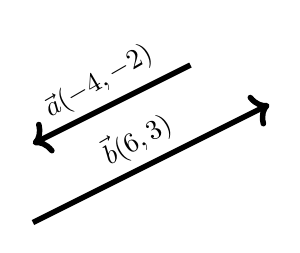
\begin{tikzpicture}[scale=0.5]
        \begin{scope}[yshift=4cm, xshift=4cm]
        \draw [->, line width = 2pt] (0, 0) -- (-4, -2) node [above, rotate=30,midway] {$\vec{a}(-4, -2)$};
        \end{scope}
    
        \draw [->, line width = 2pt] (0, 0) -- (6, 3) node [above, rotate=30, midway] {$\vec{b}(6, 3)$};
    \end{tikzpicture}
    
    코사인 유사도  -1
    \column{0.33\textwidth}

    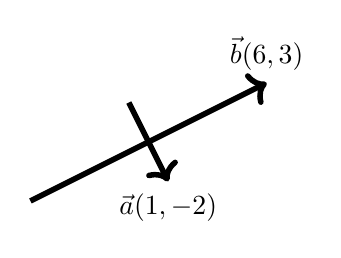
\begin{tikzpicture}[scale=0.5]
        \begin{scope}[yshift=2.5cm, xshift=2.5cm]
        \draw [->, line width = 2pt] (0, 0) -- (1, -2) node [below] {$\vec{a}(1, -2)$};
        \end{scope}
    
        \draw [->, line width = 2pt] (0, 0) -- (6, 3) node [above] {$\vec{b}(6, 3)$};
    \end{tikzpicture}
    
    코사인 유사도 0

    \column{0.33\textwidth}
    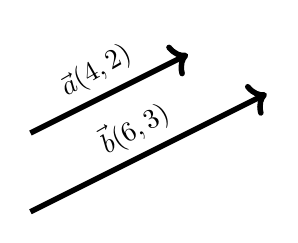
\begin{tikzpicture}[scale=0.5]
        \begin{scope}[yshift=2cm]
        \draw [->, line width = 2pt] (0, 0) -- (4, 2) node [above, rotate=30,midway] {$\vec{a}(4, 2)$};
        \end{scope}
    
        \draw [->, line width = 2pt] (0, 0) -- (6, 3) node [above, rotate=30, midway] {$\vec{b}(6, 3)$};
    \end{tikzpicture}
    
    코사인 유사도  1
\end{columns}

\end{frame}




\begin{frame}[fragile,allowframebreaks]{행렬의 덧셈과 뺄셈}
    \begin{description}
        \item[행렬] 숫자를 가로와 세로로 늘어 놓은 것 
    \end{description}

    \[ 3 \times 4 \text{행렬}, 
    \begin{bmatrix}
        3 & 4 & 0 & 10 \\
        0 & 1 & 0 & -3 \\
        -1 & 5 & 9 & 0 \\
    \end{bmatrix}
    \]

    위의 행렬은 3행 4열의 행렬 또는 $3\times 4$ 행렬이라고 함. 이 때 3행 2열의 성분은 5

    각 행과 열의 원소 끼리 덧셈 또는 뺄셈을 할 수 있으며 행렬의 크기가 같을 때만 더하거나 뺄 수 있음
\end{frame}




\begin{frame}[fragile,allowframebreaks]{행렬의 곱셈}
    행렬은 벡터의 개념이 확장된 것임. 개념 이해를 위해 다음의 행벡터 $\vec{a}$와 $\vec{b}$ 열벡터를 살펴보자. 
    
    \[\vec{a} = (-1, 2), \vec{b} = \begin{pmatrix}
        3\\2
    \end{pmatrix}\]
    
    $\vec{a}$ 와 $\vec{b}$는 각각 $1\times2 $ 과 $2\times 1$ 행렬이라고 할 수 있음.

    행렬의 곱셉은 벡터의 내적과 같음

    \begin{eqnarray*}
        \vec{a} \vec{b} &=& \langle \vec{a}, \vec{b} \rangle \\    
        \vec{a} \vec{b} &=& \begin{pmatrix}
            -1 & 2 
        \end{pmatrix} \begin{pmatrix}
            3\\
            2
        \end{pmatrix}\\
        &=& -1 \times 3 + 2 \times 2 = 1
    \end{eqnarray*}
    
    \textbf{공식}
 \begin{eqnarray*}
     \vec{a} &=& \begin{pmatrix}
         a_1 & a_2 & \ldots & a_n
     \end{pmatrix}, \vec{b} = \begin{pmatrix}
        b_1 \\
        b_2 \\
        \vdots \\
        b_n
    \end{pmatrix} \text{일 때} \\
    \vec{a} \vec{b} &=& \langle \vec{a}, \vec{b} \rangle \\    
    &=& a_1 b_1 + a_2 b_2 + \cdots + a_n b_n = \sum _{i=1} ^n a_i b_i
 \end{eqnarray*}

 \pagebreak
 \begin{columns}
     \column{0.33\textwidth}
     예제
     \begin{eqnarray*}
         \vec{a_1} &=& (-1, 2) \\
         \vec{a_2} &=& (1, 1) \\
         A &=& \begin{bmatrix}
            \vec{a_1}\\
            \vec{a_2}
        \end{bmatrix}
        =\begin{bmatrix}
            -1 & 2 \\
            1 & 1
        \end{bmatrix} \\[1em]
        \vec{b} &=& \begin{pmatrix}
            3 \\
            2
        \end{pmatrix}
     \end{eqnarray*}
     \column{0.67\textwidth}
     행렬 $A$와 열벡터 $b_1$ 은 \\
     $a_1 b_1 = \langle \vec{a_1}, \vec{b_1} \rangle = -1 \times 3 + 2 \times 2 = 1$\\
     $a_2 b_1 = \langle \vec{a_2}, \vec{b_1} \rangle = 1 \times 3 + 1 \times 2 = 5$
     \\
     곱셉 결과는 $\vec{a_1}\vec{b_1}$과 $\vec{a_2}\vec{b_1}$ 를 세로로 쌓아서 만든 열벡터가 됨

     \begin{eqnarray*}
         A \vec{b_1} &=& \begin{bmatrix}
             \vec{a_1} \\
             \vec{a_2}
         \end{bmatrix} \vec{b_1}\\
         &=& \begin{bmatrix}
            \langle \vec{a_1}, \vec{b_1} \rangle\\
            \langle \vec{a_2}, \vec{b_1} \rangle
         \end{bmatrix}\\
         &=& \begin{bmatrix}
             -1 & 2 \\
             1 & 1 
         \end{bmatrix} 
         \begin{bmatrix}
             3 \\
             2
         \end{bmatrix}\\
         &=& \begin{bmatrix}
             1 \\5
         \end{bmatrix}
     \end{eqnarray*}
 \end{columns}

 \pagebreak
\begin{eqnarray*}
    A &=& \begin{bmatrix}
        \vec{a_1}\\
        \vec{a_2}\\
        \vdots \\
        \vec{a_m}
    \end{bmatrix} = \begin{bmatrix}
        a_{11} & a_{12} & \cdots & a_{1n} \\
        a_{21} & a_{22} & \cdots & a_{2n} \\
         \vdots & \vdots & \ddots & \vdots \\
        a_{m1} & a_{m2} & \cdots & a_{mn} 
    \end{bmatrix}, \vec{b} = \begin{bmatrix}
        \vec{b_1}\\
        \vec{b_2}\\
        \vdots \\
        \vec{b_n}
    \end{bmatrix}\\
    A\vec{b} &=& \begin{bmatrix}
        \vec{a_1}\\
        \vec{a_2}\\
        \vdots \\
        \vec{a_m}
    \end{bmatrix} \vec{b} = \begin{bmatrix}
        \langle \vec{a_1}, \vec{b} \rangle\\
        \langle \vec{a_2}, \vec{b} \rangle\\
        \vdots\\
        \langle \vec{a_n}, \vec{b} \rangle\\
    \end{bmatrix} \\
    &=& \begin{bmatrix}
        \sum _{i=1}^n a_{1i}b_i \\
        \sum _{i=1}^n a_{2i}b_i \\
        \vdots\\
        \sum _{i=1}^n a_{mi}b_i 
    \end{bmatrix} =\begin{bmatrix}
        a_{1i}b_1 + a_{12}b_2 + \cdots + a_{1n}b_n \\
        a_{2i}b_1 + a_{22}b_2 + \cdots + a_{2n}b_n \\
        \vdots\\
        a_{1m}b_i + a_{m2}b_2 + \cdots + a_{mn}b_n \\
    \end{bmatrix}
\end{eqnarray*}
\pagebreak
\begin{eqnarray*}
    A &=& \begin{bmatrix}
        \vec{a_1}\\
        \vec{a_2}\\
        \vdots \\
        \vec{a_n}
    \end{bmatrix} = \begin{bmatrix}
        a_{11} & a_{12} & \cdots & a_{1n} \\
        a_{21} & a_{22} & \cdots & a_{2n} \\
         \vdots & \vdots & \ddots & \vdots \\
        a_{m1} & a_{m2} & \cdots & a_{mn} 
    \end{bmatrix}, \\
    B &=& \begin{bmatrix}
        b_1, b2, \cdots, b_l
    \end{bmatrix} = \begin{bmatrix}
        b_{11} & b_{12} & \cdots & b_{1l} \\
        b_{21} & b_{22} & \cdots & b_{2l} \\
         \vdots & \vdots & \ddots & \vdots \\
        b_{n1} & b_{n2} & \cdots & b_{nl} 
    \end{bmatrix}\\
    AB &=& \begin{bmatrix}
        \vec{a_1}\\
        \vec{a_2}\\
        \vdots \\
        \vec{a_n}
    \end{bmatrix}  \begin{bmatrix}
        b_1, b2, \cdots, b_l
    \end{bmatrix} = \begin{bmatrix}
        \langle \vec{a_1}, \vec{b_1} \rangle & \langle \vec{a_1}, \vec{b_2} \rangle & \cdots & \langle \vec{a_1}, \vec{b_l} \rangle\\
        \langle \vec{a_2}, \vec{b_1} \rangle & \langle \vec{a_2}, \vec{b_2} \rangle & \cdots & \langle \vec{a_2}, \vec{b_l} \rangle\\
        \vdots & \vdots& \cdots &\vdots\\
        \langle \vec{a_n}, \vec{b_1} \rangle & \langle \vec{a_n}, \vec{b_2} \rangle & \cdots & \langle \vec{a_n}, \vec{b_l} \rangle
    \end{bmatrix} 
\end{eqnarray*}

$AB$의 제$p$행 $q$ 열 성분은 $\langle \vec{a_p}, \vec{b_q} \rangle = \sum_{i=1} ^n a_{pi} b_{iq} = a_{p1}b_{1q} + a_{p2}b_{2q} + \cdots +  a_{pn}b_{nq}$ 임

\pagebreak
행렬의 스칼라 배

\begin{eqnarray*}
    A &=& \begin{bmatrix}
        \vec{a_1}\\
        \vec{a_2}\\
        \vdots \\
        \vec{a_m}
    \end{bmatrix} = \begin{bmatrix}
        a_{11} & a_{12} & \cdots & a_{1n} \\
        a_{21} & a_{22} & \cdots & a_{2n} \\
         \vdots & \vdots & \ddots & \vdots \\
        a_{m1} & a_{m2} & \cdots & a_{mn} 
    \end{bmatrix} \\
    kA &=& k\begin{bmatrix}
        \vec{a_1}\\
        \vec{a_2}\\
        \vdots \\
        \vec{a_m}
    \end{bmatrix} = \begin{bmatrix}
        ka_{11} & ka_{12} & \cdots & ka_{1n} \\
        ka_{21} & ka_{22} & \cdots & ka_{2n} \\
         \vdots & \vdots & \ddots & \vdots \\
        ka_{m1} & ka_{m2} & \cdots & ka_{mn} 
    \end{bmatrix}
\end{eqnarray*}

\pagebreak
$AB$ 에서 성분 $\langle \vec{a_p}, \vec{b_q} \rangle$를 정의할 수 있으려면 행렬 $A$의 열의 개수와 행렬 $B$의 개수가 같아야 함. 즉 $m\times n$ 행렬과 $n \times l$ 행렬을 곱하는 형태여야만 곱셈을 할 수 있고 그 결과는 $m \times l$ 행렬이 됨

행렬의 곱셈에서는 교환법칙 ($AB \neq BA$)이 성립하지 않음

\begin{description}
    \item[영행렬] 성분 전체가 $0$인 행렬
    \item[단위 행렬] 왼쪽 위에서 오른쪽 아래 방향으로 대각선상의 모든 성분이 1이고 그 밖의 성분은 0으로 채워진 정방행렬. 어떤 행렬이나 벡터에 단위행렬을 곱하면 그 결과가 달라지지 않고 원래 행렬이나 벡터가 나옴. 항등사상\\
    \[E = \begin{bmatrix}
        1 & 0 \\
        0 & 1
    \end{bmatrix}\]  
\end{description}

\end{frame}




\begin{frame}[fragile,allowframebreaks]{역행렬}
    \begin{description}
        \item[역행렬] 행렬에는 나눗셈 연산을 할 수 없으므로 행렬의 역수(reciprocal)를 만들어 곱셈으로 같은 효과를 낼 수 있음.  

        \[\frac{1}{2} \div \frac{3}{5} = \frac{1}{2} \times \frac{5}{3} = \frac{5}{6} \] 

        \[a \times a ^{-1} = a^{-1} \times a = 1 \]
        \[ A A^{-1} = A^{-1} A = E\]
        \item[행렬식] 역행렬의 존재 여부를 확인하기 위해 사용됨. 행렬식이 0인 경우 역행렬이 존재하지 않음. 
        \[A = \begin{bmatrix}
            a & b \\
            c & d
        \end{bmatrix}\]
        \[ \text{행렬식}= \det A = |A| \]
        \[|A| = \det A = ad-bc \]
    \end{description}

    \pagebreak
    \begin{description}
        \item[역행렬] $2\times 2$ 행렬의 역행렬은 다음과 같은 식으로 구할 수 있음
        \[A = \begin{bmatrix}
            a & b\\
            c & d 
        \end{bmatrix}\] 
        \[A^{-1} = \frac{1}{ad-bc} \begin{bmatrix}
            d & -b \\
            -c & a
        \end{bmatrix}\]
    \end{description}
    $2\times 2$  보다 큰 경우 가우스 소거법 (Gaussian elimination) 이나 여인자 전개 (cofactor expansion)과 같은 방법을 써야 함
\end{frame}




\begin{frame}[fragile,allowframebreaks]{선형 변환}
    \begin{description}
        \item[선형 변환] 수학적으로 벡터에 행렬을 곱해 또 다른 벡터를 만드는 함수. 하나의 벡터 공간에서 다른 벡터 공간으로, 벡터의 특징을 유지한 채 변환하는 방법
        \item[표준 기저] standard basis, $x$축이나 $y$축, 그리고 $z$축처럼 좌표계를 정할 수 있는 벡터의 집함
    \end{description}
    \[A = \begin{bmatrix}
        -1 & 2 \\
        1 & 1 
    \end{bmatrix}, \vec{b_1} = \begin{bmatrix}
        3\\
        2
    \end{bmatrix}, \text{일 때} A\vec{b_1}= \begin{bmatrix}
        -1 & 2 \\
        1 & 1 
    \end{bmatrix}\begin{bmatrix}
        3\\
        2
    \end{bmatrix} = \begin{bmatrix}
        1\\
        5
    \end{bmatrix}\]
    
    $A$와 $\vec{b_1}$의 표준 기저
    \begin{columns}
        \column{0.45\textwidth}
        \[A = (\vec{e_1}, \vec{e_2})\]
        \[\vec{e_1}= \begin{bmatrix}
            -1\\
            1
        \end{bmatrix}, \vec{e_2}= \begin{bmatrix}
            2\\
            1
        \end{bmatrix}\]
        \column{0.45\textwidth}
        \[\vec{b_1} = 3\begin{bmatrix}
            1\\
            0
        \end{bmatrix} + 2\begin{bmatrix}
            0\\
            1
        \end{bmatrix}\]
        \[= 3 \vec{e_x} + 2 \vec{e_y}\]
    \end{columns}
    \pagebreak
    \begin{eqnarray*}
        A\vec{b_1} &=& \begin{bmatrix}
            -1 & 2 \\
            1  & 1\\
        \end{bmatrix} \left( 3\begin{bmatrix}
            1\\
            0
        \end{bmatrix} + 2\begin{bmatrix}
            0\\
            1
        \end{bmatrix}\right) \\
        &=& 3\begin{bmatrix}
            -1 & 2 \\
            1  & 1\\
        \end{bmatrix}\begin{bmatrix}
            1\\
            0
        \end{bmatrix} + 2\begin{bmatrix}
            -1 & 2 \\
            1  & 1\\
        \end{bmatrix}\begin{bmatrix}
            0\\
            1
        \end{bmatrix} \\
        &=&3 \begin{bmatrix}
            -1 \\
            1
        \end{bmatrix} + 2 \begin{bmatrix}
            2 \\
            1
        \end{bmatrix} 
        = 3\vec{e_1} + 2 \vec{e_2} = \begin{bmatrix}
            1 \\
            5
        \end{bmatrix}
    \end{eqnarray*}

    \begin{columns}
        \column{0.5\textwidth}
        그림으로 표현한 선형 변환

        회전하거나 확대 또는 축소 할 수 있음

        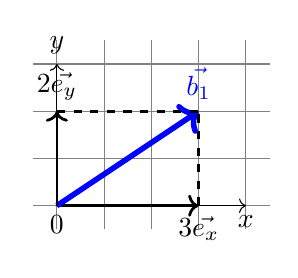
\begin{tikzpicture}% 
            [scale = 0.6]
            \draw[step=1.0,gray,thin] (-0.5,-0.5) grid (4.5,3.5);
            \node [below] at (0,0) {0};
            \draw [->,] (0,0) -- (4,0) node [below] {$x$};
            \draw [->,] (0,0) -- (0,3) node [above] {$y$};
            
            \draw [->,line width = 1pt] (0,0) -- (3,0) node [below] {$3\vec{e_x}$};
            \draw [->,blue, line width = 2pt] (0,0) -- (3,2) node [above] {$\vec{b_1}$};
            \draw [->,line width = 1pt] (0,0) -- (0,2) node [above] {$2\vec{e_y}$};
            
            
            \draw [line width = 1pt, dashed] (3,0) -- (3,2) ;
            \draw [line width = 1pt, dashed] (0,2) -- (3,2);
            
        \end{tikzpicture}
        \column{0.5\textwidth}
        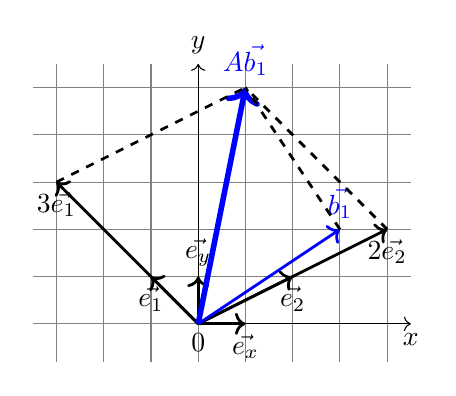
\begin{tikzpicture}% 
            [scale = 0.6]
            \draw[step=1.0,gray,thin] (-3.5,-0.8) grid (4.5,5.5);
            \node [below] at (0,0) {0};
            \draw [->,] (0,0) -- (4.5,0) node [below] {$x$};
            \draw [->,] (0,0) -- (0,5.5) node [above] {$y$};
            
            \draw [->,line width = 1pt] (0,0) -- (1,0) node [below] {$\vec{e_x}$};
            \draw [->,line width = 1pt] (0,0) -- (0,1) node [above] {$\vec{e_y}$};
            
            \draw [->,line width = 1pt] (0,0) -- (-1,1) node [below] {$\vec{e_1}$};
            \draw [->,line width = 1pt] (0,0) -- (2,1) node [below] {$\vec{e_2}$};
            
            \draw [->,line width = 1pt] (0,0) -- (-3,3) node [below] {$3\vec{e_1}$};
            \draw [->,line width = 1pt] (0,0) -- (4,2) node [below] {$2\vec{e_2}$};
            

            \draw [->,blue, line width = 1pt] (0,0) -- (3,2) node [above] {$\vec{b_1}$};
            \draw [->,blue, line width = 2pt] (0,0) -- (1,5) node [above] {$A\vec{b_1}$};            
            
            \draw [line width = 1pt, dashed] (-3,3) -- (1,5) ;
            \draw [line width = 1pt, dashed] (4,2) -- (1,5);
            \draw [line width = 1pt, dashed] (3,2) -- (1,5);
        \end{tikzpicture}


    \end{columns}
\end{frame}




\begin{frame}[fragile,allowframebreaks]{고윳값과 고유벡터}
    정방행렬 $A$가 있고 다음의 식을 만족하는 열벡터 $\vec{x}$(단$x\neq 0$)가 존재할 때 $\lambda$를 행렬 $A$ 의 고윳값(eigenvalue)이라고 하고 $\vec{x}$를 고유벡터 (eigenvector)라고 함

    \[A\vec{x} = \lambda E\vec{x}\]
    \[(A -\lambda E)\vec{x} = 0\]

    만약, $(A -\lambda E)$가 역행렬 $(A -\lambda E)^{-1}$을 갖는다면, 다음과 같이 양변에 역행렬을 곱해줄 수 있음
    \[(A -\lambda E)^{-1}(A -\lambda  E)\vec{x} = (A -\lambda E)^{-1} 0\]
    \[\vec{x} = (A -\lambda E)^{-1} 0 = 0\]
    단, $\det(A -\lambda E) = 0$

    \pagebreak
    \textbf{벡터가 회전하지 않고 확대나 축소만 할 때, 변화한 벡터의 길이 비율이 고윳값이고, 벡터의 방향이 고유 벡터가 됨}

    \begin{eqnarray*}
        \det \left( \begin{bmatrix}
            2 & 4 \\
            -1 & -3
        \end{bmatrix} - \lambda \begin{bmatrix}
            1 & 0 \\
            0 & 1 
        \end{bmatrix} \right) &=& 0\\
        \det \begin{bmatrix}
            2-\lambda & 4 \\
            -1 & -3- \lambda
        \end{bmatrix} &=& 0\\
        (2-\lambda)(-3-\lambda) - 4(-1) &=& 0\\
        \lambda ^2+\lambda -2 &=& 0\\
        (\lambda +2)(\lambda -1)&=&0
    \end{eqnarray*}


\pagebreak
    
\textbf{case 1} $\lambda = -2 $
    \[ (A-(-2)E)\vec{x} = \begin{bmatrix}
        2-(-2)& 4\\
        -1&-3-(-2)
    \end{bmatrix}\vec{x} = \begin{bmatrix}
        4 & 4\\
        -1 & -1
    \end{bmatrix}\vec{x} =0\]
이 식을 만족하는 해가 고유벡터 $\vec{x}$임. 

$\vec{x} = \begin{bmatrix}
    \alpha\\
    \beta
\end{bmatrix}$라고 가정하고 $\begin{bmatrix}
    4& 4\\
    -1 & -1
\end{bmatrix}\begin{bmatrix}
    \alpha\\
    \beta
\end{bmatrix} = \begin{bmatrix}
    0\\
    0
\end{bmatrix}$ 을 풀면 $\alpha + \beta = 0$ 이 나옴

상수 $t$를 가정하고 $\alpha = t$ 그리고 $\beta = -t\begin{bmatrix}
    0\\
    0
\end{bmatrix}$라고 풀어 쓸수 있음.

$\vec{x} = t\begin{bmatrix}
    1\\
    -1
\end{bmatrix}$ 이고 $x$는 $\begin{bmatrix}
    1\\
    -1
\end{bmatrix}$의 상수 배가 됨

\pagebreak

\textbf{case 2} $\lambda = 1$
\[ (A-(1)E)\vec{x} = \begin{bmatrix}
    2-(-1)& 4\\
    -1&-3-(-1)
\end{bmatrix}\vec{x} = \begin{bmatrix}
    1 & 4\\
    -1 & -4
\end{bmatrix}\vec{x} =0\]
이 식을 만족하는 해가 고유벡터 $\vec{x}$임. 

$\vec{x} = \begin{bmatrix}
    \alpha\\
    \beta
\end{bmatrix}$라고 가정하고 $\begin{bmatrix}
    1 & 4\\
    -1 & -4
\end{bmatrix}\begin{bmatrix}
    \alpha\\
    \beta
\end{bmatrix} = \begin{bmatrix}
    0\\
    0
\end{bmatrix}$ 을 풀면 $\alpha + 4\beta = 0$ 이 나옴

정리하면 $\alpha = -4 \beta$ 이고, 이를 풀면 $\alpha = t$ 그리고 $\beta = -\frac{1}{4}t$ 가 됨

$x = t \begin{bmatrix}
    1\\
    -\frac{1}{4}
\end{bmatrix}=t \frac{1}{4}\begin{bmatrix}
    4\\
    -1
\end{bmatrix}$ 이 되어 $\vec{x}$는 $\begin{bmatrix}
    4 \\
    -1
\end{bmatrix}$ 의 상수 배가 됨

고유값과 이에 대응하는 고유벡터는 각각 두 개씩 있음

\pagebreak

인공지능 알고리즘 중 비지도 학습에서 주성분 분석 (PCA, Principal Component Analysis)라는 기법을 쓰는데, 이 때 고윳값과 고유벡터를 활용함. 기여율을 사용하여 각 주성분(고유벡터에 대응하는 고윳값을 전체 고윳값들의 총합으로 나눈 값)이 데이터를 얼마나 잘 설명하는지 평가하는 척도로 사용


\end{frame}

\section{확률과 통계}

\begin{frame}[fragile, allowframebreaks] {확률}
    \begin{description}
        \item[확률] 어떤 사건이 우연히 발생할 가능성을 표현한 것. $P$
    \end{description}
    \[\text{확률} = \frac{\text{어떤 사건이 발생할 수 있는 경우의 가짓수}}{\text{모든 경우의 가짓수}}\]

    \begin{description}
        \item[조합] combination, 서로 다른 $n$개로부터 중복 없이 $k$개를 골라내는 경우의 수
    \end{description}
    \[ ~_nC_k = \frac{n \cdot (n-1)\cdots (n-k+1)}{1\cdot 2\cdot~ \cdots~\cdot(k-1)\cdot k}\]
    
    예: 트럼프 카드에서 다섯 장의 카드를 동시에 뽑았을 때, 다섯 장 모두가 하트인 경우는 몇 가지인가. $~_{13}C_5$

    \pagebreak

    \begin{description}
        \item[여사건] complimentary event,  사건 $A$가 발생할 확률이 $P$일 때, 사건 $A$의 여사건, $\bar{A}$가 발생할 확률
    \end{description}
    \[P(\bar{A}) = 1 - P\]

    예: 트럼프 카드에서 4장의 카드를 동시에 뽑았을 때, 적어도 1장이 스페이드인 경우의 확률. $1- \frac{~_{39}C_4}{~_{52}C_4}$

    \pagebreak

    \begin{description}
        \item[합사건] 사건 $A$와 사건 $B$가 동시에 발생하는 사건: $A \cap B$ ($A$ and $B$)
        \[P(A \cap B ) = P(A)P(B)\]
        \item[곱사건] 사건 $A$와 사건 $B$중에서 어느 한쪽이 발생할 사건 $A \cup B$ ($A$ or $B$)
        \[P(A \cup B) = P(A)+P(B) - P(A \cap B)\] 
    \end{description}

    \def\firstcircle{(0,0) circle (1.5cm)}
\def\secondcircle{(0:2cm) circle (1.5cm)}

\colorlet{circle edge}{blue!50}
\colorlet{circle area}{blue!20}

\tikzset{filled/.style={fill=circle area, draw=circle edge, thick},
    outline/.style={draw=circle edge, thick}}

\setlength{\parskip}{5mm}
% Set A and B

\begin{columns}
    \column{0.25\textwidth}
    
\begin{tikzpicture}[scale = 0.45]
    \begin{scope}
        \clip \firstcircle;
        \fill[filled] \secondcircle;
    \end{scope}
    \draw[outline] \firstcircle node {$A$};
    \draw[outline] \secondcircle node {$B$};
    \node[anchor=south] at (current bounding box.north) {$A \cap B$};
\end{tikzpicture}

\column{0.25\textwidth}
    
%Set A or B but not (A and B) also known a A xor B
\begin{tikzpicture}[scale = 0.45]
    \draw[filled, even odd rule] \firstcircle node {$A$}
    \secondcircle node{$B$};
    \node[anchor=south] at (current bounding box.north) {$\overline{A \cap B}$};
\end{tikzpicture}

\column{0.25\textwidth}
    
% Set A or B
\begin{tikzpicture}[scale = 0.45]
    \draw[filled] \firstcircle node {$A$}
                    \secondcircle node {$B$};
    \node[anchor=south] at (current bounding box.north) {$A \cup B$};
\end{tikzpicture}

\column{0.25\textwidth}

% Set A but not B
\begin{tikzpicture}[scale = 0.45]
    \begin{scope}
        \clip \firstcircle;
        \draw[filled, even odd rule] \firstcircle node {$A$}
                                     \secondcircle;
    \end{scope}
    \draw[outline] \firstcircle
                    \secondcircle node {$B$};
    \node[anchor=south] at (current bounding box.north) {$A - B$};
\end{tikzpicture}
\end{columns}

\end{frame}


\begin{frame}[fragile, allowframebreaks] {확률변수와 확률분호}
\begin{description}
    \item[확률변수] random variable, 어떤 변수 $X$를 사용할 때 확률 $P(X)$의 확률로 구할 수 있다면 $X$는 확률변수임. 예: 주사위를 두 번 던져 합이 2가 될 확률 $P(X_2 = 2) = \frac{1}{6} \cdot \frac{1}{6} = \frac{1}{36}$
    \item[이산확률변수] discrete random variable, 확률변수 중에 연속되지 않고 셀 수 있을 만큼 흩어진 경우를 말함. 예: 주사위에 적힌 숫자, 사건이 일어나는 시행 횟수
    \item[연속확률변수] continuous random variable, 값이 특정 범위 내에서 실수 형태로 존재하며, 소수점 이하까지 내려가는 경우. 예: 몸무게, 경과 시간과 같이 끊김 없이 연속적으로 이어지는 값
    \item[이산확률분포] discrete probability distribution, 어떤 사건의 이산확률변수가 $X$일 때, 그에 대한 확률 $P$는 이산확률분포 $f(x)$를 따름 \[P(X)=f(x)\]
\end{description}


주사위를 두 개 던졌을 때 숫자의 합과 그에 대한 확률

\begin{tabular}{*{12}{|c}|}\hline
    $X_2$ & 2 & 3& 4& 5 & 6& 7& 8& 9& 10 & 11 & 12 \\ \hline
    $P(X_2)$ & $\frac{1}{36}$ & $\frac{2}{36}$ & $\frac{3}{36}$ & $\frac{4}{36}$ & $\frac{5}{36}$ & $\frac{6}{36}$ & $\frac{5}{36}$ & $\frac{4}{36}$ & $\frac{3}{36}$ & $\frac{2}{36}$ & $\frac{1}{36}$  \\ \hline
\end{tabular}

\pagebreak
\begin{columns}
    \column{0.5\textwidth}
    주사위가 하나일 때 히스토그램
\begin{tikzpicture}[scale=0.5]
    \begin{axis}[ymin=0, ymax=25, ybar, bar width = 25pt, xlabel={$X_1$},
        ylabel={$P(X_1)[\%]$}]
    \addplot plot coordinates {  (1, 16.6) (2, 16.6) (3, 16.6) (4, 16.6) (5, 16.6) (6,16.6) };
    \legend{$f(x)=P(X_1)$};
    \end{axis}
    \end{tikzpicture}

    균등분포
    \column{0.5\textwidth}
    주사위가 두 개일 때 히스토그램
    \begin{tikzpicture}[scale=0.5]
        \begin{axis}[ymin=0, ymax=18, ybar, bar width = 17pt, xlabel={$X_1$},
            ylabel={$P(X_1)[\%]$}]
        \addplot plot coordinates {  (2, 1/36*100) (3, 2/36*100) (4, 3/36*100) (5, 4/36*100) (6, 5/36*100) (7, 6/36*100) (8, 5/36*100) (9, 4/36*100) (10, 3/36*100) (11, 2/36*100) (12, 1/36*100) };
        \legend{$f(x)=P(X_1)$};
        \end{axis}
        \end{tikzpicture}

        종형 곡선 (bell curve)
\end{columns} 

\pagebreak

\begin{description}
    \item[연속확률분포] 어떤 사건의 연속확률변수가 $X$일 때, 그에 대한 확률 $P$는 연속확률분포 $f(x)$를 지정한 $X$의 구간 안에서 적분한 값과 같음 \[P (a \leq X \leq b ) = \int_a^b f(x)\text{d}x\]
\end{description}
\vspace{-1.5em}
\pgfplotsset{
  myplot/.style={
    width=16cm, height=5cm,
    samples=50, smooth, no marks,
    xlabel={키 $H[m]$}, ylabel={$P(H)[\%]$},
   %xlabel style={at={(1,0)}, anchor=north west},
    %ylabel style={rotate=-90, at={(0,1)}, anchor=south east},
    legend style={draw=none, fill=none}
  }
}

\begin{center}
    

\begin{tikzpicture}[scale=0.7,
  >=stealth,
  every node/.style={rounded corners},
  declare function={
    normalpdf(\x,\mu,\sigma)=
    (2*pi*\sigma^2)^(-0.5)*exp(-(\x-\mu)^2/(2*\sigma^2));
  },
  hplot/.style={ycomb, mark=o, dashed}]

  \begin{axis}[myplot, xmin=1.4, xmax=2]

    \addplot[domain=1.72:1.75, draw=none, fill=green]
    {normalpdf(x,1.7,0.1)} \closedcycle;
    \addplot[smooth, thick, domain=1.2:2.2]
    {normalpdf(x,1.7,0.1)}
    node[pos=0.35, pin={left:$\mu=1.7$, $\sigma^2=0.1^2$}] {};
    \addplot[hplot, samples at={1.7}] {normalpdf(x,1.7,0.1)};
    
    \node[anchor=north west] at (axis description cs: 0.02, 0.95)
    {$f(x)=P(H)$};

    \coordinate (p0) at (axis cs: 1.73, 1);
    \node[fill=green, draw=none] (p1)
    at (axis description cs: 0.78, 0.75)
    {\footnotesize $\displaystyle \int_{172}^{175}f(x)$};
    \path[o->] (p0) edge[out=45, in=-90] (p1);

  \end{axis}

\end{tikzpicture}
\end{center}

연속확률분포 종류: 정규분포 (normal distribution), 지수분포 (exponential distribution), 스튜던트 t 분포 (student's t-distribution), 파레토 분포 (Pareto distribution), 로지스틱 분포 (logistic distribution)


\end{frame}



\begin{frame}[fragile] {결합확률과 조건부확률}
    \begin{description}
        \item[결합확률] 사건 $A$와 사건 $B$가 서로 독립된 사건일 때, 두 사건의 결합확률(동시에 일어날 확률)은 다음과 같음 \[P(A\cap B)= P(A, B) = P(A)P(B)\]
        \item[조건부 확률] 사건 $B$가 일어났을 때, 사건 $A$가 일어날 조건부 확률은 다음과 같음 \[P(A|B)=\frac{P(A\cap B)}{P(B)}\]
        \[P(A\cap C) = P(A) \cdot P(\bar{B})\]\[P(C) = P(A\cap \bar{B})+P(\bar{A} \cap B)\]
    \end{description}
\end{frame}



\begin{frame}[fragile] {기댓값}
    \begin{description}
        \item[기댓값] 모든 이산확률변수 $X$에 대한 기댓값 $E(X)$는 다음과 같음. 이때, 확률은 $P(X)$ \[E(X)=\sum P(X)\cdot X \]
    \end{description}

    $X$와 $Y$가 서로 독립된 확률변수이고 $k$는 상수라고 할 때 다음 식이 성립함
    \begin{enumerate}
        \item $E(k) = k$: 상수의 기댓값은 상수
        \item $E(kX) = kE(X)$: 확률변수를 상수 배하면 기댓값도 상수배가 됨
        \item $E(X+Y) = E(X) + E(Y)$ : 확률변수의 합의 기댓값은 각 기댓값의 함과 같음
        \item $X$ 와 $Y$ 가 서로 독립일 때 $E(XY) = E(X) \cdot E(Y)$ : 독립적인 확률변수의 곱에 대한 기댓값은 각 기댓값의 곱과 같음
    \end{enumerate}
\end{frame}



\begin{frame}[fragile,allowframebreaks] {평균과 분산 그리고 공분산}
    \begin{description}
        \item[평균값] $n$개의 확률변수가 각각 $x_1, x_2, \ldots, x_n$이라는 값을 가질 때 평균값 $\bar{x}$는 다음과 같음 \[\bar{x}= \sum_{k_1}^n \frac{1}{n} \cdot x_k = \frac{1}{n}\sum _{k_1}^{n} x_k\]
        \item[분산] $n$개의 확률변수가 각각 $x_1, x_2, \ldots, x_n$ 이라는 값을 가지고 평균값이 $\bar{x}$일 때 분산 $\sigma^2$은 다음과 같음 \[\sigma^2 = \frac{1}{n}\sum_{k=1}^{n} (x_k-\bar{x})^2\]
        \item[표준편차] 편차는 $+$와 $-$ 같은 부호를 갖고 있음. 평균을 기준으로 떨어진 정도를 나타냄. $\sigma$는 다음과 같음. \[\sigma = \sqrt{\sigma^2} = \sqrt{\frac{1}{n}\sum_{k=1}^{n} (x_k-\bar{x})^2}\] 
    \end{description}
    \pagebreak

    \begin{description}
            \item[공분산] 두 확률변수의 상관관계를 확인할 때 사용. 두 가지 데이터에 대한 $n$조의 확률변수 $(X, Y) = \left\{ (x_1, y_1),  (x_2, y_2), \ldots,  (x_n, y_n) \right\}$이 있다고 가정함. $X$의 평균이 $\mu_x$이고 $Y$의 평균이 $\mu_y$라고 할 때 공분산은 $Cov(X, Y)$ 다음과 같음 \[Cov(X,Y) = \frac{1}{n}\sum_{k=1}^{n} (x_k - \mu_x)(y_k - \mu_y)\] 
    \end{description}
\end{frame}



\begin{frame}[fragile] {상관계수}
    \begin{description}
        \item[상관계수] 확률변수 $X$와 $Y$의 분산이 양수이고 각각의 표준편차가 $\sigma_X, \sigma_Y$ 공분산이 $\sigma_{XY}$라고할 때의 상관계수는 다음과 같음 (이때, $-1\leq \rho \leq 1$) \[\rho = \frac{\sigma_{XY}}{\sigma_X\sigma_Y}\] 
    \end{description}
    
    공분산을 상관계수로 변환하였기 때문에 상관계수 끼리 강약을 비교할 수 있음
\end{frame}



\begin{frame}[fragile] {최대가능도추정}
    \begin{description}
        \item[최대가능도추정] maximum likelihood estimation. 가장 그럴듯하게 값을 추정.\\
        최대가능도추정이란 어떤 파라미터 $\theta$의 값을 추정하는 방법이며, $\theta$에 대한 가능도 함수 $L(\theta)$ 을 최대로 만드는 $\theta$을 찾는 것. 이때의 $\theta$에 대한 추정값은 다음 방정식을 만족함\[\frac{\text{d}L(\theta)}{\text{d}\theta}= 0\]
    \end{description}

    이산확률분포의 식은 확률의 곱으로 표현이 되기 때문에 미분이 쉽지 않음. 가능도함수에 자연로그를 붙여 주어 로그가능도함수 $\log_e L(\theta)$를 만들면 됨
    \[\frac{\text{d}}{\text{d}\theta}\log_e L(\theta)=0\]
\end{frame}

\section{선형회귀}

\begin{frame}[fragile] {선형모델의 변수}
    \begin{description}
        \item[목적변수] objective variable 추정하고 싶은 값
        \item[종속변수] dependent variable 추정하고 싶은 값
        \item[설명변수] explanatory variable 추정하는 데 필요한 정보
        \item[독립변수] independent variable 추정하는 데 필요한 정보
    \end{description}
\end{frame}

\begin{frame}[fragile] {데이터 척도}
    \begin{tabular}{p{5em} | p{5em} |p{6cm} }
        분류 & 척도 & 설명 \\ \hline
        \multirow{2}{*}{질적 데이터} & 명목척도 (nominal scale) & 분류나 구별을 하기 위한 척도. 더미 변수라고도 함 (예: 남성 0, 여성 1) \\ \cline{2-3}
        & 서열척도 (ordinal scale) & 대소 관계만 의미가 있는 척도 (예: 나쁨: 0, 보통: 1, 좋음: 2)\\ \hline
        \multirow{2}{*}{양적 데이터} & 등간척도 (interval scale) & 간격에 의미가 있는 변수. 덧셈, 뺄셈만 의미가 있음 (예: 서기)\\ \cline{2-3}
        & 비율척도 (ratio scale) & 비례에도 의미가 있는 변수. 덧셈, 뻴셈, 곱셈, 나눗셈 전체에 의미가 있음. (예: 속도, 키, 체중)\\ 
    \end{tabular}
\end{frame}

\begin{frame}[fragile] {선형회귀 모델}
    \begin{description}
        \item[회귀 모델] 하나의 목적변수(종속변수)를 하나 이상의 설명변수(독립변수)로 기술한 관계식. 계수(가중치)는 일반적으로 $w_0, w_1, \ldots, w_n$로 표현하고 설명변수는 일반적으로 $x_1, x_2, \ldots, x_n$로 표현함
    \end{description}
    \begin{eqnarray*}
        y&=& w_0 + \sum_{k=1}^l w_k x_k\\
        y &=& w_0 +w_1x_1+w_2x_2+\ldots+w_n x_n\\
        \begin{bmatrix}
            y_1\\
            y_2\\
            \vdots\\
            y_n
        \end{bmatrix} &=& \begin{bmatrix}
            1 & x_{11} & x_{12} & \cdots & x_{1l} \\
            1 & x_{21} & x_{22} & \cdots & x_{2l} \\
            \vdots & \vdots \vdots & \ddots & \vdots \\
            1 & x_{n1} & x_{n2} & \cdots & x_{nl} \\
        \end{bmatrix}
        \begin{bmatrix}
            w_1\\
            w_2\\
            \vdots\\
            w_n
        \end{bmatrix}\\
        y&=&XW
    \end{eqnarray*}
\end{frame}

\begin{frame}[fragile,allowframebreaks] {최소제곱법으로 파라미터 도출}
    \begin{description}
        \item[최소제곱법] least squared method 수치 데이터들을 1차함수와 같은 특정 함수를 사용하여 근사적으로 표현하는 방법. 수치 데이터 값과 함수의 결과값 사이에 오차가 최소가 되도록 하는 것. 이 과정에서 오차가 가장 작게 나오는 가중치를 찾으면 이를 모델식의 계소로 사용함.
    \end{description}


    


\begin{columns}
    \column{0.4\textwidth}
    \vspace{1em}
\begin{filecontents}{lsm.dat}
    xd yd
    0.5  8.7
    0.8  7.5
    1.1  7.1
    1.5  6.8
\end{filecontents}
    
    \pgfplotstableread{lsm.dat}
    \loadedtable
    
    \begin{tikzpicture}[scale=0.6]
    \begin{axis}[
      xlabel={Distance (km)},
      ylabel={Price ($\times 10^3$)},
      legend style ={draw=none}]
    \addplot [mark =*, only marks] table [y=yd, x=xd]{lsm.dat};
    \addlegendentry{Price per Dist}
    
    
    \addplot [no markers, thick, red]
          table [y={create col/linear regression={y=yd}}] {lsm.dat}
          node [anchor=east] {$\pgfmathprintnumber[precision=2, fixed zerofill]
          {\pgfplotstableregressiona} \cdot \mathrm{Weight} +
          \pgfmathprintnumber[precision=1]{\pgfplotstableregressionb}$};
    
    \end{axis}
    \end{tikzpicture}
    
\column{0.6\textwidth}
실제 데이터와 추세선 간의 거리의 차

\begin{eqnarray*}
    D&=& \sum_{l=1} ^{29} |y_l - (w_0 +w_1 x_l)|\\
    &=& \sum_{l=1} ^{29} (y_l - (w_0 +w_1 x_l)^2
\end{eqnarray*}
\end{columns}

\pagebreak
\begin{eqnarray*}
    D &=& \sum_{l=1} ^{29} (y_l - (w_0 +w_1 x_l)^2\\
    D &=& (8.7-(w_0 +0.5w_1))^2 +(7.5-(w_0 +0.8w_1))^2 \\
    &&+ (7.1-(w_0 +1.1w_1))^2 + (6.8-(w_0 +1.5w_1))^2   \\
    D &=& 4w_0^2 + 4.35 w_1^2 +7.8 w_0w_1 -60.2w_0 - 56.72w_1 + 228.59
\end{eqnarray*}

\pagebreak 

이때 $D$가 최솟값을 가지려면 $w_0$과 $w_1$로 편미분했을 때 값이 0이 되어야 함. 그러므로 다음과 같은 식을 만들 수 있음

\begin{eqnarray*}
    \frac{\delta D}{\delta w_0} &=& 8 w_0 + 7.8 w_1 - 60.2 = 0\\
    \frac{\delta D}{\delta w_1} &=& 8.7 w_0 + 7.8 w_1 - 56.72 = 0\\
\end{eqnarray*}

연립방정식을 풀면

\[-1.8037 x + 9.2836 \]

\pagebreak

일반적으로는 목적변수 $Y$, 설명변수 $X_1, X_2, \ldots, X_l$ 그리고 모델식 $f(X_1, X_2, \ldots, X_l)$이라고 할 때 최소제곱법을 적용하는 과정은 오차의 제곱합 $D$를 최소화하는 $f(X_1, X_2, \ldots, X_l)$를 구하는 문제임.

$n$개의 데이터 세트에서 k번째의 데이터를 $(x_k1, x_k2, \ldots, x_kl, y_k)$ 오차의 제곱합은 다음과 같은 식으로 표현할 수 있음.

\begin{eqnarray*}
    D&=& \sum_{k=1} ^{n} (y_k - f(x_{k1}, x_{k2}, \cdots, x_{kl})^2
\end{eqnarray*}

모델 식은 다음과 같음.\vspace{-1em}
\begin{eqnarray*}
    f(x_k1, x_k2, \ldots, x_kl) &=& \sum_{m=1} ^{l} w_mx_{km}+w_0
\end{eqnarray*}
{\footnotesize \textbf{가중치$(w_0, w_1, \dots, w_l)$를 변화시키면서 함수 $D(w_0, w_1,\ldots, w_l)$d이 최소가 되는 값을 만드는 가중치의 조합을 찾기!!  각 가중치의 편미분이 0이 되는 해 찾기}}

\end{frame}

\begin{frame}[fragile,allowframebreaks] {정규화로 과학습 줄이기}
    샘플 데이터
    \begin{center}
        \begin{filecontents}{sample.dat}
            xd yd
            -4	-44
            -3.5	-25
            -3	-8
            -2.5	0
            -2	10
            -1.5	14
            -1	15
            -0.5	5
            0	8
            0.5	20
            1	10
            1.5	11
            2	-8
            2.5	1
            3	2
            3.5	10
            4	35
            \end{filecontents}
            
            \pgfplotstableread{sample.dat}
            \loadedtable
            
            \begin{tikzpicture}[scale=0.6]
            \begin{axis}[axis lines=left]
            \addplot [mark =*, only marks] table [y=yd, x=xd]{sample.dat};            
            \end{axis}
            \end{tikzpicture}
    \end{center}

\pagebreak

\begin{columns}

    

    \column{0.5\textwidth}

    \begin{description}
        \item[일반화 능력] generalization ability, 약간의 노이즈는 허용하면서 전체적인 데이터의 특성은 잘 반영한 식
    \end{description}
    \begin{tikzpicture}[scale=0.6]
        \begin{axis}
            \draw[line width=1pt, red] (axis cs: -4,-44) .. controls (axis cs: 0,100) and (axis cs: 2,-74) .. (axis cs: 4,40) ;
            
            \addplot [mark =*, only marks] table [y=yd, x=xd]{sample.dat};  
        \end{axis}
    \end{tikzpicture}
    
   
    
    \column{0.5\textwidth}
    \begin{description}
        \item[과학습/과적합] overfitted, 주어진 데이터에 너무 정확히 들어맞아 지나치게 복잡하게 표현된 상태
    \end{description}
\vspace{1em}
    \begin{tikzpicture}[scale=0.6]
        \begin{axis}
            \addplot [mark =*] table [y=yd, x=xd]{sample.dat};
        \end{axis}
    \end{tikzpicture}
    
   
\end{columns}

\pagebreak
\begin{description}
    \item[정규화] 선형회귀에서 과학습을 피하는 방법. 모델이 복잡해질 수록 일종의 패널티를 적용하여 과학습을 억제 
\end{description}

정규화 방법: $L1$ 정규화, $L2$ 정규화, Norm과 같음

선형회귀 모델 : $y = w_0 + \sum_{k=1}^l w_k x_k$

정규화를 위해 추가할 항: $\lambda E(w)$

\pagebreak

$L1$ 정규화에서는 파라미터의 $L1$ norm에 계수를 곱한 다음과 같은 항을 사용
\[\lambda E(w) =\sum_{k=1}^l |w_k| \]
최소제곱오차 식$D=\sum_{k=1}^n ( y_k - f(x_{k1}, x_{k2}, \ldots, x_{kl}))^2$에 추가

Lasso 회귀
\[D=\sum_{k=1}^n ( y_k - f(x_{k1}, x_{k2}, \ldots, x_{kl}))^2 + \lambda E(w) \]

\pagebreak
$L2$ 정규화에서는 파라미터의 $L2$ norm에 계수를 곱한 다음과 같은 항을 사용
\[\lambda E(w) =\sum_{k=1}^l |w_k^2|\]
그리고 $L1$ 정규화를 할 때와 같이 최소제곱오차를 구하는 식에 항을 추가
\[D=\sum_{k=1}^n ( y_k - f(x_{k1}, x_{k2}, \ldots, x_{kl}))^2 + \lambda E(w)\]

$L2$ 정규화에서는 $L1$정규화와 달리 절댓값을 사용하지 않음. 미분이 상대적으로 쉬움. 이렇게 정규화된 선형회귀를 Ridge 회귀라고 함

$L1$ 정규화는 $L2$정규화는 기존의 모델식에 조합해서 쓸 수 있고 이 둘을 조합할 수 도 있음. 그렇게 만들어진 회귀 모델을 Elastic Net이라고 함

scikit-learn에서는 특별히 지정하지 않은 한 기본적으로 $\lambda = 1.0$으로 계산함. 정규화 강약을 조정하려면 $\lambda$를 조절
\end{frame}

\begin{frame}[fragile,allowframebreaks] {모델 평가}

    모델을 검증하기 위한 데이터 세트를 만드는 방법
    \begin{description}
        \item[홀드아웃 교차 검증법] holdout cross validation, 하나의 데이터 세트를 학습용 데이터와 테스트용 데이터 두 가지로 나누는 방법
        \item[k-분할 교차 검증법] k-fold cross validation, 데이터 세트를 $k$개로 분할한 다음, $k$번에 걸쳐 학습 데이터와 테스트 데이터의 조합을 바꿔쓰는 방법
    \end{description}
    \pagebreak

    모델의 성능은 시각화를 통해 눈으로도 확인할 수 있는 잔차 (residual) 그래프에 표시

    \begin{description}
        \item[잔차] 추정된 회귀식과 실제 데이터 사이의 차이 
    \end{description}

    회귀식을 $y= w_0 + \sum_{k=1}^l w_k x_k$라고 $i$번째의 잔차를 $e_i$라고 할 때 잔차를 구하는 식은 다음과 같음
    \[e_i = y_i - \left(w_0 + \sum_{k=1}^l w_k x_{ki}\right)\]

\pagebreak
    $n$개의 데이터가 있을 때 평균제곱오차와 결정계수는 다음과 같은 식으로 구할 수 있음
    \begin{eqnarray*}
        MSE &=& \frac{1}{n}\sum_{i=1}^n (y_{실측값i} -y_{예측값i})^2 \\
        R^2 &=& 1 -\frac{MSE}{\frac{1}{n}\sum_{i=1}^n (y_{실측값i} - \bar{y_{실측값i}})^2}, (0 \leq R^2 \leq 1)
    \end{eqnarray*}

    $R^2$ 의 분모는 $y$의 분산이고, $\bar{y_{실측값i}}$은 $y_{실측값i}$의 평균을 뜻함. 이 지표는 0 이상 1 이하의 값을 갖고 있으며 1에 가까울 수록 잘 맞는 모델임.
\end{frame}

\section{Classification}
\begin{frame}[fragile, allowframebreaks]{로지스틱 회귀}
    \begin{description}
        \item[로지스틱 회귀] Logistic regression, 1이 될 확률 $p$이고 0이 될 확률이 $1-p$인 이산확률분포를 사용하여 1이나 0의 값을 확륙적으로 얻는  방법. 이산확률분포로는 베르누이 분포 (Bernoulli distribution) 등이 있음
    \end{description}

$x$가 실수 입력값이고 $y={0, 1}$이 출력값일 때, 출력값은 반드시 0과 1중 하나가 나옴. 이때, 출력값 $y=1$이 되는 조건부확률 $p(y=1|x;\theta)$는 다음과 같음. 이때 $\theta$는 실수 파라미터임
\[p(y=1|x;\theta) = \frac{1}{1+exp(-\theta^T x)}\]

\pagebreak

$p(\theta)=\frac{1}{1+exp(-\theta)}$를 로지스틱 함수라고 함 치역은 0에서 1이고 평균 값인 0.5가 되는 함수. 시그모이드 함수로 소개됨

\begin{center}
    \begin{tikzpicture}[scale=0.5]
        \begin{axis}[axis lines=middle, ytick={0,0.1,...,1},          ylabel={$p(\theta)$},
        xlabel={$\theta$}, width = 15cm , height=7cm  ]
        \addplot[smooth,domain=-10:10,purple,very thick] {1/(1+exp(-x))};
        \addplot [no marks]coordinates {(-10,0.5) (10,0.5)};
        \node at(axis cs: 5,0.7) {$p(\theta)=\frac{1}{1+exp(-\theta)}$};
        \end{axis}
    \end{tikzpicture}
\end{center}

\pagebreak

이 함수의 정의역은 실수 전체로 $\theta>0$일 때 $y=1$이 될 확률 $p(\theta)$가 0.5보다 커지는 특징이 있음. 이 특징을 사용하여 어떤 대상을 분류할 때 사용함

학습데이터로 쓸 데이터 세트 $(x_i, y_i)$가 $1\leq i \leq m$만큼 주어졌다고 가정할 때 다음과 같은 식이 성립함
\begin{eqnarray*}
    p_i (y= y_i | x_i; \theta) \geq 0.5 \text{일때, } y_i = 1\\
    p_i (y= y_i | x_i; \theta) < 0.5 \text{일때, } y_i = 0
\end{eqnarray*}

\end{frame}

\begin{frame}[fragile, allowframebreaks]{목적함수}
    확률표현을 $p_i (y= y_i | x_i; \theta)$와 같이 간단히 표현한 후, 목적 함수 $J(\theta)$를 최소로 만드는 $\theta$를 구한다고 할 때, 다음과 같은 목적 함수를 만들 수 있음

    \[J(\theta) = \frac{1}{2m}\sum_{i=1}^{m}(p_{x_i} - y_i)^2\]

    일반적으로는 이 식을 최소화하는 $\theta$를 구하기 위해 전개해야 함. 이 경우는 $0 \leq p_{x_i} \leq 1$이고, $y_i$는 0 또는 1만 나온다는 사실을 알고 있기 때문에 다음과 같은 손실 함수 $L(\theta)$로 바꿔서 계산하는 것이 효과적임

    \[L(\theta) = - \sum_{i=1}^m (y_i log(p_{x_i}) + (1-y_i)\log(1-p{x_i}))\]


    \pagebreak

    $L2$ 정규화를 적용한 로그 목적함수는 다음과 같음. 이때 $\lambda$는 정규화의 강도를 나타내는 파라미터임

    \[L(\theta) = - \sum_{i=1}^m (y_i log(p_{x_i}) + (1-y_i)\log(1-p{x_i})) + \frac{1}{2\lambda}\sum_{j=1}^n \theta_j^2\]

    다중 클래스 분류 (multi-class classification)의 경우 one-vs-rest 기법을 사용하여 여러 개의 이진 클래스 분류기 문제로 나눠서 해결함. ($y=i, y\neq i$)
\end{frame}

\begin{frame}[fragile]{정밀도, 재현율, F값}
    
    \begin{tabular}{|c| c| p{4cm}| p{4cm}|}\hline
        && \multicolumn{2}{c|}{예측 결과}\\ \cline{3-4}
        && Positive & False \\ \hline
        실제 & True& 진양성, True positive, TP & 위음성, False negative, FN \\ \cline{2-4}
        결과& 거짓 & 위양성, False Positive, FP & 진음성, True negative, TN\\ \hline
        
    \end{tabular}
    
    \begin{description}
        \item[정밀도]  \[\text{Precision} = \frac{TP}{TP+FP}\]
        \item[재현율] \[\text{Recall} = \frac{TP}{TP+FN}\]
        \item[F 값] \[F = \frac{2\times \text{Recall} \times \text{Precision}}{\text{Recall} + \text{Precision}} = \frac{2TP}{2TP+FN+ FP}\]
    \end{description}

\end{frame}
    
\section{Neural Networks}

\begin{frame}[fragile]{모델}
    \begin{center}
        
    \begin{tikzpicture}
        \node  [thick, align=left,circle, draw,  pin={[pin edge ={<-,ultra thick}, pin distance= 22pt]125:{b(bias)}}, pin ={[pin edge ={<-, ultra thick, pin distance= 22pt}, line width = 2pt]225:{x(input)}}, pin ={[pin edge ={->, ultra thick, pin distance= 22pt}, line width = 2pt]0:{a(output)}}]  at (0,0) {활성화 $\sigma$ \\ $wx+b \rightarrow \sigma(wx+b)$};
            \end{tikzpicture}
        \end{center}

\end{frame}



\begin{frame}[fragile, allowframebreaks]{비선형 변환}

    \begin{columns}
        \column{0.45\textwidth}
        \begin{equation*}
            \varsigma_a(x) = \frac{1}{1+\exp (-ax)}
        \end{equation*}
        \begin{tikzpicture}[scale=0.7]
            \begin{axis}[ymax=1, xmin=-20, xmax=20,domain=-20:20,axis lines=middle]
            \addplot[smooth,purple,very thick] {1/(1+exp(-x))};
            \node at (250, 50) {0.5};
            \end{axis}
        \end{tikzpicture}
        \column{0.45\textwidth}
        \begin{eqnarray*}
            \varphi (x) = \max (0, x ) = \begin{cases}
                x & (x > 0) \\
                0 & (x \leq 0)
            \end{cases} 
        \end{eqnarray*}
        \begin{tikzpicture}[scale=0.7]
            \draw[->] (-3,0) -- (3,0) node[right] {x};
            \draw[->] (0,0) -- (0, 3) node[left] {y};
            \draw[line width = .1cm, purple]  (-3,0) -- (0,0) -- (3,3) ;
        \end{tikzpicture}
    \end{columns}


\pagebreak

   \begin{columns}       
    \column{0.45\textwidth}
    선형 분리가 가능한 경우\vspace{1em}

    \begin{tikzpicture}[scale=0.6]
        \begin{axis}
        \addplot [mark =o, only marks] coordinates  {(1,1) (1.2, 2) (1.5, 3) (2,2) (2.2, 3) (3,3) (3.3, 4.5) (4,4) (4.4, 5.3) (5,5)   };
        \addplot [mark =x, thick,only marks] coordinates  {(1.5,0.5) (2.2, 1.5) (2.5, 1.5) (3,1.7) (3.5, 2) (3.8, 2) (3.8,3) (4,3) (4.3, 3.5) (4.6,3.9)    };
        \addplot [mark=none, dashed, line width=1pt, red] coordinates {(1, 0.7) (5, 4.8)};
        \end{axis}
    \end{tikzpicture}
    
    
    \column{0.45\textwidth}
선형 분리가 불가능한 경우 \vspace{1em}

\begin{tikzpicture}[scale=0.6]
    \begin{axis}
    \addplot [mark =o, only marks] coordinates  {(1,1.5)(1.1,1.5) (1.2, 2.5)(1.4,3.5) (1.5, 3.5) (2,3.5) (2.2, 3.3)(2.5, 3.3) (3,2.5) (3.2,2.5) (3.3, 2) (3.8, 2.5) (4,3)(4.1,3) (4.4, 4) (5,5.2)   };
    \addplot [mark =x, thick,only marks] coordinates  {(1.5,1) (1.7, 2.7) (2.1, 2.8) (2.2, 2.5) (2.5, 1.5) (3,1.5) (3.5, 1.3) (3.8, 1.3) (3.8,1) (4,1.5) (4.3, 1.5) (4.6,2.5) (4.7,2.7) (4.9,3)  };
    \draw[line width=1pt, red] (axis cs: 1, 0.7) .. controls (axis cs: 2,8) and (axis cs: 3,-4) .. (axis cs: 5,5) ;
    \end{axis}
\end{tikzpicture}


\end{columns}


\vspace{3em}
비선형 변환 활성화 함수를 사용하여 분리 할 수 있도록 만들어야 함


\end{frame}


\begin{frame}[fragile, allowframebreaks]{순전파}

    \begin{center}
    \begin{neuralnetwork}[height=4]
        \newcommand{\xneuralf}[2]{$x^{0}_#2$}
        \newcommand{\y}[2]{$a_#2$}
        \newcommand{\hfirst}[2]{\small $h^{1}_#2$}
        \newcommand{\hsecond}[2]{\small $h^{2}_#2$}
        \inputlayer[count=3, bias=false, title=Input layer, text=\xneuralf]
        \hiddenlayer[count=2, bias=true, title=Hidden layer 1, text=\hfirst] \linklayers
        \hiddenlayer[count=2, bias=true, title=Hidden layer 2, text=\hsecond] \linklayers
        \outputlayer[count=2, title=Output layer, text=\y] \linklayers
    \end{neuralnetwork}
\end{center}
{\footnotesize 
 \begin{columns}
     \column{0.15\textwidth}
     입력값\\
     \[\Scale[2]{x_{\beta}^{\alpha}}\]
     $\alpha$ : 계층번호\\
     $\beta$ : 노드번호
     
     \column{0.15\textwidth}
     출력값\\
     \[\Scale[2]{a_{\beta}^{\alpha}}\]
     $\alpha$ : 계층번호\\
     $\beta$ : 노드번호

     \column{0.3\textwidth}
     가중치\\
     \[\Scale[2]{w_{\beta\gamma}^{\alpha}}\]
     $\alpha$ : 다음 계층번호\\
     $\beta$ : 다음 계층 노드번호\\
     $\gamma$ : 이전 계층의 노드번호
     
     \column{0.3\textwidth}
     바이어스\\
     \[\Scale[2]{b_{\beta}^{\alpha}}\]
     $\alpha$ : 다음 계층번호\\
     $\beta$ : 다음 계층 노드번호
     
     
     
    \column{0.15\textwidth}
    활성화 함수\\
    \[\Scale[2]{\sigma_{\alpha}}\] 
    $\alpha$ : 계층번호 
     
     
     
 \end{columns}
 }

 \pagebreak

 최초의 입력층에서는 별다른 처리를 하지 않음
 \[x_{1}^0 = a_1^0, x_{2}^0 = a_2^0\]

 은닉층의 입력값은 다음과 같이 표현됨
 \begin{eqnarray*}
    x_1^1 &=& w_{11} ^1 a_1^0 + w_{12} ^1 a_2^0 + w_{13} ^1 a_3^0 + b_1^1 \\
    x_2^1 &=& w_{21} ^1 a_1^0 + w_{22} ^1 a_2^0 + w_{23} ^1 a_3^0 + b_2^1   
 \end{eqnarray*}

 행렬로 표현하면 다음과 같음
     \[x^1 = \begin{pmatrix}
         x_1^1\\
         x_2^1
     \end{pmatrix}, \qquad W^1 = \begin{pmatrix}
        w_{11}^1 & w_{12}^1 & w_{13}^1 \\
        w_{21}^1 & w_{22}^1 & w_{23}^1 
     \end{pmatrix}, \qquad a^0 = \begin{pmatrix}
         a_1^0\\
         a_2^0\\
         a_3^0
     \end{pmatrix}, \qquad b^1 = \begin{pmatrix}
        b_1^1\\
        b_2^1
     \end{pmatrix} \]
     \[x^1 = W^1 a^0 + b^1\]
 
\pagebreak
은닉층의 출력값 ($\sigma$함수는 시그모이드 함수로 가정)
\begin{eqnarray*}
    a_1^1 & =& \sigma_1(x_1^1)    \\
    a_2^1 & =& \sigma_1(x_2^1)    
\end{eqnarray*}

 예를 들어 $x_1^1 = 0$일때 시그모이드 함수를 사용하면 $a_1^1 = \sigma_1(0) = 0.5$가 됨


은닉층에서 출력층으로 정보 전달

\[x^2 = \begin{pmatrix}
    x_1^2\\
    x_2^2\\
    x_3^2
\end{pmatrix}, \qquad W^2 = \begin{pmatrix}
   w_{11}^2 & w_{12}^2  \\
   w_{21}^2 & w_{22}^2  \\
   w_{31}^2 & w_{32}^2 
\end{pmatrix}, \qquad a^1 = \begin{pmatrix}
    a_1^1\\
    a_2^1
\end{pmatrix}, \qquad b^2 = \begin{pmatrix}
   b_1^2\\
   b_2^2\\
   b_3^2
\end{pmatrix} \]
\[x^2 = W^2 a^1 + b^2\]

\pagebreak

\begin{description}
    \item[softmax 함수] $n$차원의 실수 벡터 $\vec{x}=(x_1, x_2, \ldots, x_n)$이 있다고 가정할 때, 다음 식에서 $n$ 차원의 실수 벡터 $\vec{y}=(y_1, y_2, \ldots, y_n)$을 결괏값으로 내는 함수를 softmax함수라고 부름 
\end{description}
\[y_i = \frac{\exp(x_i)}{\exp(x_1)+\exp(x_2)+\cdots+\exp(x_n)}\qquad (1\leq i \leq n)\]

softmax를 사용하면 결괏값을 확률적인 표현으로 만들 수 있음

2계층에서 적용된 softmax 함수를 $\sigma_2$라고 할 때, 이 함수의 결과로 나오는 확률 $a_1^2, a_2^2, a_3^2$는 다음과 같이 표현됨
\[a_1^2=\sigma_2(x_1^2), \qquad a_2^2=\sigma_2(x_2^2), \qquad a_3^2=\sigma_2(x_3^2)\]

$a_1^2, a_2^2, a_3^2$ 중에서 가장 큰 값이 나오는 카테고리가 판별의 결과

\end{frame}


\begin{frame}[fragile, allowframebreaks]{손실 함수}
    가중치와 바이어스를 조정할 때는 손실 함수의 값이 최소가 되도록 만들어야 함

    \begin{description}
        \item[손실함수] 신경망이 출력한 값과 실제 값과의 오차에 대한 함수 
    \end{description}

    다양한 손실함수가 있음. 그 중 평균제곱오차 (MSE, mean squred error) $E$는 다음과 같이 구함. 이때, $t$는 정답 레이블 $y$는 신경망의 출력
    \[E= \frac{1}{2}\| t- y\|^2\]

    \pagebreak
    
    \begin{block}{예시}
        3계층 신경망에서 2계층의 출력 $y^2$가 $y^2=(0.1w, 0.5w, 1-0.6w)$이고 정답 $t$는 $t=(0, 1, 0)$이라고 할 때 평균 제곱오차 $E$를 구하고 이 값을 최소로 만드는 $w$를 구하시오        
    \end{block}
\begin{eqnarray*}
    E &=& \frac{1}{2}((0-0.1w)^2+ (1-0.5w)^2 + (0-1(1-0.6w))^2 )\\
    E &=& 0.31w^2 - 1.1w +1
\end{eqnarray*}

평균제곱오차를 최소화시키려면 $w$로 미분했을 때의 값이 0이 되도록 해야 함 {\scriptsize(답 $w\approx 1.774$)}
\[\frac{\text{d}E}{\text{d}w} = 0.62w-1.1 = 0\]

softmax의 결과 예시 2
\begin{tabular}{*{11}{|c}|}\hline
    & 0 & 1 & 2 & 3 & 4 & 5 & 6 & 7 & 8 &  9  \\ \hline
    출력층 y & 0.01 & 0.02 & 0.05 & 0.02 & 0.67 & 0.13 & 0.05 & 0.01 & 0.01 & 0.03 \\ \hline
    레이블 t & 0 & 0 & 0 & 0 & 1 & 0 & 0 & 0 & 0 & 0 \\ \hline
\end{tabular}

이때의 평균제곱오차는 다음과 같이 구함

(정답인 경우 1 그 외는 0으로 표기하는 one-hot  기법 사용)
\begin{eqnarray*}
    E&=&\frac{1}{2} ( (0-0.01)^2+(0-0.02)^2+(0-0.05)^2+(0-0.02)^2+(1-0.67)^2\\
    && +(0-0.13)^2+(0-0.05)^2+(0-0.01)^2+(0-0.01)^2+(0-0.03)^2) \\
    &=& 0.0664
\end{eqnarray*}

\pagebreak

\begin{block}{교차 엔트로피}
    \[E = - \sum t \log_e y \]

    평균제곱오차에서 사용한 one-hot 표현법은 0 과 1 뿐이 없기 때문에 교차 엔트로피를 손실함수로 사용함
\end{block}
\vspace{1em}
\begin{columns}
    \column{0.45\textwidth}
    
    \begin{tikzpicture}[scale=0.7]
        \begin{axis}[domain=0.01:2, samples = 100, grid, no markers]        \addplot +[line width =2pt] (\x,{ln(\x)});
        \draw [line width =1pt](axis cs:-1,0) -- (axis cs:3,0);
        
        \end{axis}
        
    \end{tikzpicture}
    
    \column{0.45\textwidth}

 {\footnotesize 그래프를 보면 $y$가 1일 때 $E=0$이 나오고 $y$가 0에 가까워질수록 $E$의 값은 0보다 작아짐. 0에 가까워질 수록 음수가 나오는데 이것을 양수로 만들기 위해 교차 엔트로피의 손실 함수에 마이너스 부호를 붙임. 
 
 출력층의 활성화 함수로 softmax함수를 사용할 때 출력값은 $0\leq y\leq 1$과 같은 확률 표현됨. 결과 $y$는 1을 넘지 않으므로 $\log_e y >0$이 되지 않음
 }


\end{columns}

\end{frame}


\begin{frame}[fragile, allowframebreaks]{경사하강법}
    입력층, 은닉층 출력층이 많아질 수록 평균제곱오차를 최소화하기 위해 고려해야 하는 변수의 수가 기하급수적으로 많아짐 (예: 입력층 3, 은닉층2, 출력층 3개 일때 변수 17개)

    \begin{description}
        \item[경사하강법] 함수의 그래프를 따라 움직이면서 기울기를 조사하고 이때 구한 기울기의 값이 작아지는 방향으로 조금씩 이동하는 방법 
    \end{description}

    {\centering \begin{tikzpicture}[scale=0.5,
        every edge/.style = {draw, -{Triangle[angle=60:1pt 3,flex]},
                                     bend right=11, blue,ultra thick},
        every edge quotes/.style = {font=\scriptsize, inner sep=1pt, 
                                    auto, sloped}
                                    ]
        \fill (0,0) circle[radius=3pt];
        \path[name path=C] foreach \i in {4, 8, 16, 22, 28}
                {(0,0) circle[draw=red!\i, x radius=2*\i mm, y radius=\i mm, rotate=-5]};
        \foreach \i in  {4, 8, 16, 22, 28}
            \draw[line width=11.2/\i, draw=white!\i!gray]
                (0,0) circle[x radius=2*\i mm, y radius=\i mm, rotate=-5];
        \path[name path=V] (-4,2.4) .. controls + (0,-2) and + (-2,0) .. (0,0);
        %
        \draw [name intersections={of=C and V, sort by=C, name=A}]
                (A-5) edge ["${w[0]}$"] (A-4)
                (A-4) edge ["${w[1]}$"] (A-3)
                (A-3) edge ["${w[2]}$"] (A-2);
    \end{tikzpicture}
    }

    \pagebreak
    경사하강법 수식

    \[\
    \frac{\text{d}f(x)}{\text{d}x} = \lim_{\Delta \rightarrow 0} \frac{\Delta f(x)}{\Delta x} =  \lim_{\Delta \rightarrow 0} \frac{f(x+h)-f(x)}{h}
    \]
    $h= \Delta x$라고 가정하면
    \[\frac{\text{d}f(x)}{\text{d}x} = \lim_{\Delta \rightarrow 0} \frac{f(x+\Delta x)-f(x)}{\Delta x} \]
    $\Delta x$ 가 충분히 작은 값이라고 한다면 $\lim_{\Delta \rightarrow 0} $에 따라서 다음과 같은 근사식이 됨
    \[\frac{\text{d}f(x)}{\text{d}x} \approx \lim_{\Delta \rightarrow 0} \frac{f(x+\Delta x)-f(x)}{\Delta x} \]
    양변에 $\Delta x$을 곱해 전개하면 다음과 같이 됨 (근사공식)
    \[\frac{\text{d}f(x)}{\text{d}x}\Delta x \approx \lim_{\Delta \rightarrow 0} f(x+\Delta x)-f(x) \]

    함수 $f(x)$에 대해 $x$에 $\Delta$만큼의 변화를 주었을 때 $f(x)$의 변화량을 $\Delta f$이라고 하면 다음과 같이 정리할 수 있음
    \[\Delta f(x) = f(x+\Delta x)-f(x) \]

    앞의 식에 대입하면 다음과 같이 정리됨
    \[\Delta f(x) \approx \frac{\text{d}f(x)}{\text{d}x} \Delta x \]

    원하는 것은 $\Delta f(x)$가 음이 되는 방향으로 $\Delta x$를 조금씩 이동하며 최솟값을 찾아야 함.
    
    \pagebreak

    최솟값을 찾을 조건
    \begin{itemize}
        \item 접선의 기울기 ($\frac{\text{d}f(x)}{\text{d}x} \Delta x$)가 음일때 $\Delta x$가 양이라면 $\Delta f(x)$는 음
        \item 접선의 기울기 ($\frac{\text{d}f(x)}{\text{d}x} \Delta x$)가 양일때 $\Delta x$가 음이라면 $\Delta f(x)$는 음
    \end{itemize}

    다음과 같은 수식이 성립한다면 함수의 최솟값을 찾기 위해 그래프를 타고 내려갈 수 있음
    \[\Delta x = -\eta\frac{\text{d}f(x)}{\text{d}x} \]

    이때  $\eta$를 학습률(learning rate)이라고 부르고 너무 크거나 너무 작으면 최솟값에 이르지 못할 수 있음

    \pagebreak

    이동하기 전후의 위치를 $x_{old}$, $x_{new}$라고 하면 다음과 같이 표현할 수 있음 (갱신식)
    \[\Delta x = x_{new}- x_{old}\]

    앞의 식에 대입하면 다음과 같음
    \[x_{new} = x_{old} -\eta\frac{\text{d}f(x)}{\text{d}x} \]

    다변수 함수인 경우의 경사하강법 식은 다음과 같이 정리됨 (우변의 괄호안을 손실 함수 $E$의 기울기라고 표현함)
    \[E = -\eta\left(\frac{\partial E}{\partial w_{11}^1} , \frac{\partial E}{\partial w_{21}^1}, \frac{\partial E}{\partial w_{31}^1}, \cdots \right)\]

    \pagebreak
    
    경사하강법을 사용하여 모든 학습 데이터의 오차 계산을 해야하면 학습시간이 너무 오래 걸리는 문제가 있음.
    
    확률적 경사하강법을 사용하여 이 문제를 해결함.

    학습데이터 중 $N$의 데이터를 골라 학습시킨 후 그 결과로 나온 손 함수에 경사하강법을 적용하여 가중치를 구하는 방법

    이 과정을 반복하면 $N$개의 데이터마다 가중치를 갱신할 수 있게 되는데, 이때 처리하는 $N$개의 데이터 개수를 배치 사이즈라고 함

    학습 데이터를 몇 차례 다시 사용하면서 정확도를 높일 수 있는데, 이때 반복하는 횟수를 에포크(epoch)라고 함
\end{frame}


\begin{frame}[fragile, allowframebreaks]{오차역전파법}
    손실 함수의 기울기를 구하는 것은 쉽지 않은 일임. 가중치나 바이어스 변수가 너무 많고, 이를 미분할 때도 계산량이 너무 많기 때문임

    손실 함수의 기울기를 좀 더 쉽게 구할 수 있는 방법이 필요함

    오차역전파법이 이를 개선하기 위해 등장

    \begin{columns}
        \column{0.45\textwidth}
        \begin{block}{순전파방식}
            입력값에 가중치를 곱하고, 그 값을 다음 계층으로 전달하는 과정을 반복하는 방식
        \end{block}
        \column{0.45\textwidth}
        \begin{block}{역전파방식}
            출력값과 정답 사이의 오차를 먼저 구한 후, 그 정보를 바탕으로 바로 직전 단계의 계층의 가중치와 바이어스를 조정하는 방식
        \end{block}
    \end{columns}

    \vspace{1em}
    손실함수는 평균제곱오차 식을 사용하고 닉층의 활성화 함수로 표준 시그모이드 함수를 사용

\begin{block}{우리의 목표}
    함수의 기울기를 구하기 위해 다변수 함수의 기울기$\left(\frac{\partial E}{\partial w_{11}^1} , \frac{\partial E}{\partial w_{21}^1}, \frac{\partial E}{\partial w_{31}^1}, \cdots \right)$를 최소화하는 것

    일반화하면 $\frac{\partial E}{\partial w_{kj}^l}$을 최소화하는 것
\end{block}

    \pagebreak

    개념 도식
\vspace{-2em}
\begin{center}  

 \begin{tikzpicture}[ ->,>=stealth',shorten >=1pt,auto,node distance=2.5cm,
        thick,main node/.style={circle}]

\node[main node, draw] (1) {$x_j^{l-1}; ~~ a_j^{l-1}$};
\node[main node, draw] (2) [right of=1, node distance=4cm] {$x_k^l;~~~ a_k^l$};
\node[main node] (j) [below left of=1] {$j^{th}$ node};
\node[main node] (l) [above of=1] {$l-1$ layer};
\node[main node] (ll) [above of=2] {$l$ layer};

\node[main node] (b) [node distance=2cm, above left of=2] {$b_k^l$};
\node[main node] (w) [below left of=2] {$w_{jk+1}^l\times a_{j+1}^{l-1}$};
\node[main node] (k) [below right of=2] {$k^{th}$ node};


\path
(1) edge [loop above] node {activation function} (1)
(j) edge (1) 
(b) edge (2)
(w) edge (2)  
(k) edge (2) 
(1) edge node [above] {$~~w_kj^l \times a_j^{l-1}~~$} (2)
(2) edge [loop above] node {activation function} (2)

(2) edge [loop above] node {activation function} (2)

;      
\end{tikzpicture}
\end{center}


\pagebreak

미분의 연쇄법칙 적용
\[\frac{\partial E}{\partial w_{kj}^l} = \frac{\partial E}{\partial x_k^l}\frac{\partial x_k^l}{\partial w_{kj}^l}\]
$x_k^l$을 풀어 쓰면 다음과 같음
\[x_k^l = w_{kl}^l a_1^{l-1} + w_{k2}^l a_2^{l-1} + \cdots  + w_{kj}^la_j^{l-1} + \cdots + b_k^l\]

$x_k^l$를 $w_{kl}^l$로 미분하면 다음과 같은 식을 얻음
\[\frac{\partial x_k^l}{\partial w_{kj}^l} = a_j^{l-1}\]

앞의 식에 적용하면 다음과 같은 결과를 얻음
\[\frac{\partial E}{\partial w_{kj}^l} = \frac{\partial E}{\partial x_k^l} a_j^{l-1} \]

$a_j^{l-1}$는 직전 계층의 출력이기 때문에 쉽게 얻을 수 있음. 

이해를 위해 오차 $\delta_k^l$를 $\delta_k^l=\frac{\partial E}{\delta x_k^l}$로 바꿔서 다음과 같이 표현

\[ \frac{\partial E}{\delta x_k^l} = \delta_k^l a_j^{l-1}\]

$\delta_k^l$는 계층에 따라 구하는 방법이 다름
\begin{itemize}
    \item case1: 마지막 계층 일때
    \item case2: 마지막 계층이 아닐 때
\end{itemize}
\end{frame}

\begin{frame}[fragile, allowframebreaks] {마지막 계층일 때 $\delta _k^l$}
    혼돈을 막기 위해 $l$을 $L$로 바꿈 $\rightarrow \delta_k^L$
    \[\delta _k^L = \frac{\partial E}{\delta x_k^L} \]
    연쇄법칙을 적용
    \[\delta_k^L = \frac{\partial E}{\delta x_k^L} = \frac{\partial E}{\partial a_k^L}\frac{\partial a_k^L}{\delta x_k^L}\]
    
    $\frac{\partial a_k^L}{\delta x_k^L}$는 다음과 같이 표현할 수 있음
    \[\frac{\partial a_k^L}{\delta x_k^L} = \frac{\partial \varsigma (x_k^L)}{\partial x_k^L} = \varsigma'(x_k^L)\]

    $\frac{\partial E}{\partial a_k^L}$는 다음과 같이 표현할 수 있음
    \[\frac{\partial E}{\partial a_k^L} = \frac{\partial \frac{1}{2} (a_k^L-y_k)^2 }{\partial a_K^L} = (a_k^L - y_k) \]

    정리하면 다음과 같은 식을 만들 수 있음
    \begin{eqnarray*}
        \delta_k^L &=& \frac{\partial E}{\partial x_k^L} = \frac{\partial E}{\partial a_k^L}\frac{\partial a_k^L}{\delta x_k^L} \\
        &=& \frac{\partial \frac{1}{2} (a_k^L-y_k)^2 }{\partial a_K^L}\varsigma' (x_k^L) \\
        &=& (a_k^L - y_k) \varsigma' (x_k^L) 
    \end{eqnarray*}

    $a_k^L$는 마지막 계층일 때의 출력, $y_k$는 마지막 계층일 때의 정답 레이블, 그리고 $\varsigma' (x_k^L)$ 는 마지막 계층일 때의 입력을 활성화 함수에 대입 후 미분한 것

    \pagebreak 

Case 1: 마지막 계층일 때의 $\delta_k^L$ 의 도식화

    \begin{center}  
        \begin{tikzpicture}[ ->,>=stealth',shorten >=1pt,auto,node distance=2.5cm,
               thick,main node/.style={circle}]
       
       \node[main node, draw] (1) {$x_{j~~}^{L}; ~~ a_{k~~}^{L}$};
       \node[main node, draw] (2) [below of=1] {$x_{k+1}^L;~~~ a_{k+1}^l$};
       \node[main node] (3) [left of=1] {};
       \node[main node] (4) [left of=2] {};
       \node[main node] (5) [right of= 1] {정답};     
       \node[main node] (6) [right of= 2] {레이블};    
       \node[main node] (7) [ right of= 1, node distance = 1.5cm] {};
       \node[main node] (8) [ left of= 1, node distance = 1.5cm] {};

       \path
       %(3) edge [loop above] node {activation function} (1)
       (3) edge (1) 
       (4) edge (2)
       (1) edge [<->] node [above] {오차} (5)
       (2) edge [<->] node [above] {오차} (6)
       (8) edge [<-, bend left=90] node [above] {$\delta _k^L$를 구할 수 있음} (7)       
       ;      
       \end{tikzpicture}
       \end{center}

\end{frame}

\begin{frame}[fragile, allowframebreaks] {마지막 계층이 아닐 때 $\delta _k^l$}
   $\delta_k^l$를 구하는 방법,
   
   다음 식의 값을 구하는 것이 목표임: $\delta_k^l = \frac{\partial E}{\partial x_k^l}$

   \[\delta_1^2 = \frac{\partial E}{\partial x_1^3}\frac{\partial x_1^3}{\partial a_1^2}\frac{\partial a_1^2}{\partial x_1^2} + \frac{\partial E}{\partial x_2^3}\frac{\partial x_2^3}{\partial a_1^2}\frac{\partial a_1^2}{\partial x_1^2}  + \frac{\partial E}{\partial x_3^3}\frac{\partial x_3^3}{\partial a_1^2}\frac{\partial a_1^2}{\partial x_1^2}\]

   
   \textbf{각 항에 나오는 첫 번째 부분}
   
   $\frac{\partial E}{\partial x_1^3}$ 은 노드의 오차 $\delta_j^l$의 정에 의해서 $\frac{\partial E}{\partial x_1^3} = \delta _1^3$과 같이 표현할 수 있음
   \[\frac{\partial E}{\partial x_1^3} = \delta _1^3, \qquad \frac{\partial E}{\partial x_2^3} = \delta _2^3, \qquad \frac{\partial E}{\partial x_3^3} = \delta _3^3 \]
   \pagebreak

   \textbf{각 항에 나오는 두 번째 부분}
    $\frac{\partial x_1^3}{\partial a_1^2}$은 $x_1^3 = a_1^2 w_{11}^3 +  a_2^2 w_{12}^3 + b_1^3$를 적용하면 $\frac{\partial x_1^3}{\partial a_1^2} = w_{11}^3$과 같이 표현할 수 있음
    \[\frac{\partial x_1^3}{\partial a_1^2} = w_{11}^3, \qquad \frac{\partial x_2^3}{\partial a_1^2} = w_{21}^3, \qquad \frac{\partial x_3^3}{\partial a_1^2} = w_{31}^3 \]

    \textbf{각 항에 나오는 세 번째 부분}
    $\frac{\partial a_1^2}{\partial x_1^2}$의 경우를 보면, $a_1^2 = \varsigma(x_1^2)$
    \[\frac{\partial a_1^2}{\partial x_1^2} = \frac{\partial \varsigma(x_1^2)}{\partial x_1^2} = \varsigma' (x_1^2)\]

    \pagebreak

    정리하면 $\delta_1^2$는 다음과 같이 정리할 수 있음
    \begin{eqnarray*}
        \delta_1^2 &=& \frac{\partial E}{\partial x_1^3}\frac{\partial x_1^3}{\partial a_1^2}\frac{\partial a_1^2}{\partial x_1^2} + \frac{\partial E}{\partial x_2^3}\frac{\partial x_2^3}{\partial a_1^2}\frac{\partial a_1^2}{\partial x_1^2}  + \frac{\partial E}{\partial x_3^3}\frac{\partial x_3^3}{\partial a_1^2}\frac{\partial a_1^2}{\partial x_1^2} \\
        &=& \delta_1^3 w_{11}^3 \varsigma' (x_1^2) + \delta_2^3 w_{21}^3 \varsigma' (x_1^2) + \delta_3^3 w_{31}^3 \varsigma' (x_1^2) \\
        &=& (\delta_1^3 w_{11}^3  + \delta_2^3 w_{21}^3  + \delta_3^3 w_{31}^3 )\varsigma' (x_1^2)
    \end{eqnarray*}

    이 식을 일반화하면 다음과 같이 표현할 수 있음
    \begin{eqnarray*}
        \delta_k^l &=& (\delta_1^{l+1} w_{1k}^{l+1}  + \delta_2^{l+1} w_{2k}^{l+1}  + \cdots + \delta_m^{l+1} w_{mk}^{l+1} )\varsigma' (x_k^l) \\
        \delta_k^l &=& \sum_{i=1}^m (\delta_i^{l+1} w_{ik}^{l+1})\varsigma' (x_k^l) 
    \end{eqnarray*}

    $m$은 $l+1$ 계층에 있는 노드의 개수

    \pagebreak

    Case 2: 마지막 계층이 아닐 때의 $\delta_k^l$의 도식화

    \begin{center}  
        {\scalebox{0.9}{
        \begin{tikzpicture}[scale=0.7, ->,>=stealth',shorten >=1pt,auto,node distance=2cm,
               thick,main node/.style={circle}]
       
       \node[main node, draw] (1) {$\delta_k^{l-1}$};
       \node[main node, draw] (2) [below of=1] {$\delta_{k+1}^{l-1}$};
       \node[main node, draw] (3) [below of=2] {$\delta_{k+2}^{l-1}$};
       \node[main node, draw] (o) [above right of=2] {$\delta_{k}^{l}$};
       \node[main node, draw] (o1) [below of=o, node distance= 2.5cm] {$\delta_{k+1}^{l}$};
       \node[main node] (4) [left of=1] {입력층};
       \node[main node] (5)[left of=2] {입력층};
       \node[main node] (6)[left of=3] {입력층};
       \node[main node] (7)[right of=o] {출력층};
       \node[main node] (8)[right of=o1] {출력층};
       \node[main node] (9) [above of = 1, node distance=1cm] {$l-1$ layer} ;
       \node[main node] (10) [above of = o, node distance = 1.5cm] {$l$ layer} ;

       \path
       %(3) edge [loop above] node {activation function} (1)
       (o) edge (1) 
       (o) edge (2)
       (o) edge (3)
       (o1) edge (1) 
       (o1) edge (2)
       (o1) edge (3)   
       (1) edge (4)
       (2) edge (5)
       (3) edge (6)
       (o) edge (7)
       (o1) edge (8)   
       ;      
       \end{tikzpicture}}}
       \end{center}

    \pagebreak
    $l$계층의 $\delta_k^l$에서 $l-1$계층의 오차 $\delta_k^{l-1}$를 구할 수 있음
    \[
        \delta_k^l = 
       \begin{cases}
        (a_k^l - y_k)\varsigma'(x_k^L) & \text{L}\\
        \sum_{i=1}^m (\delta_i^{l+1}w_{ik}^{l+1})\varsigma'(x_k^l) & l
     \end{cases}
    \]     

    바이어스를 구하는 식은 가중치를 구하는 식과 같음

    $l-1$계층의 출력이 1일 때 $a_j^{l-1}=1$ 이 됨
    \[\frac{\partial E}{\partial b_k^l} = \delta _k^l \]
\end{frame}

\begin{frame}[fragile, allowframebreaks] {오차역전파법 공식 정리}
    \begin{eqnarray*}
        \frac{\partial E}{\partial w_{kj}^l} &=& \delta_k^l a_j^{l-1} \\
        \frac{\partial E}{\partial b_k^l} &=& \delta_k^l j^{l} \\
    \end{eqnarray*}
    \[
        \delta_k^l = 
       \begin{cases}
        (a_k^l - y_k)\varsigma'(x_k^L) & l \text{이 마지막 계층일 때}\\
        \sum_{i=1}^m (\delta_i^{l+1}w_{ik}^{l+1})\varsigma'(x_k^l) & l \text{이 마지막 계층이 아닐 때}
     \end{cases}
    \]
    {\footnotesize
    \begin{columns}
        \column{0.45\textwidth}
        $E$: 손실함수\\
        $w_{kj}^l$: $l$계층 $k$번째 노드의 $l-1$계층 $j$번째 노드로부터의 가중치\\
        $\delta_k^l$: $l$계층 $k$번째 노드의 오차\\
        $a-j^{l-1}$: $l-1$계층 $j$번째 노드의 출력\\
        \column{0.45\textwidth}
        $b_k^l$: $l$계층 $k$번째 노드의 바이어스\\
        $y_k$: $k$번째 노드의 정답 레이블\\
        $\varsigma(x_k^l)$: 활성화 함수\\
        $m$: $l+1$계층의 노드 개수(시그모이드 함수 등)
    \end{columns}
    }
\end{frame}

\begin{frame}[fragile, allowframebreaks] {오차역전파법 수식과 순서 정리}
    \begin{alertblock}{1. 손실 함수를 구한 후, 그 값을 최소화하기 위한 $w$와 $b$를 구함\\~}
        수식\\
        \[E= \frac{1}{2}\| \vec{t}- \vec{y}\|^2, \qquad \vec{y} = W\vec{x}+\vec{b}\]
        \begin{columns}
            \column{0.45\textwidth}
            $t$: 정답 레이블\\
            $y$: 신경망의 출력\\
            $W$: 가중치\\
            \column{0.45\textwidth}
            $x$: 출력\\
            $b$: 바이어스\\
        \end{columns}
        \vspace{1em}

        \textbf{문제점:} 최소화하고 싶은 변수 $w$와 $b$의 개수가 너무 많아 미분할 때 0이 되는 연립방정식을 풀기가 어려움
    \end{alertblock}

    \pagebreak
    \begin{alertblock}{2. 경사하강법을 사용하여 손실 함수의 값이 작아지는 방향을 확인\\~}
        수식\\
        \[w_{new} = w_{old} -\eta\frac{\partial E}{\partial w_{old}} ,\qquad b_{new} = b_{old}-\eta \frac{\partial E}{\partial b_{old}}\]
        \begin{columns}
            \column{0.45\textwidth}
            $w_{new}$: 이동 후의 가중치\\
            $w_{old}$: 이동 전의 가중치\\
            $\eta$: 학습률\\
            \column{0.45\textwidth}
            $b_{new}$: 이동 후의 바이어스\\
            $b_{old}$: 이동전의 바이어스\\
        \end{columns}

        \vspace{1em}
        \textbf{문제점:} 값을 움직일 양을 구하기 위해 $\frac{\partial E}{\partial w}$ 와 $\frac{\partial E}{\partial b}$를 계산하기에는 너무 많은 미분 대상이있어서 어려움
    \end{alertblock}

    \pagebreak
    \begin{alertblock}{3. 오차역전파법을 사용하여 가중치를 결정\\~}
        수식
        \begin{eqnarray*}
            \frac{\partial E}{\partial w_{kj}^l} = \delta_k^l a_j^{l-1} ,
            \qquad \frac{\partial E}{\partial b_k^l} = \delta_k^l j^{l} \\
        \end{eqnarray*}
        \[
            \delta_k^l = 
           \begin{cases}
            (a_k^l - y_k)\varsigma'(x_k^L) & l \text{이 마지막 계층일 때}\\
            \sum_{i=1}^m (\delta_i^{l+1}w_{ik}^{l+1})\varsigma'(x_k^l) & l \text{이 마지막 계층이 아닐 때}
         \end{cases}
        \]

        {\footnotesize
        \begin{columns}
            \column{0.45\textwidth}
            $E$: 손실함수\\
            $w_{kj}^l$: $l$계층 $k$번째 노드의 $l-1$계층 $j$번째 노드로부터의 가중치\\
            $\delta_k^l$: $l$계층 $k$번째 노드의 오차\\
            $a-j^{l-1}$: $l-1$계층 $j$번째 노드의 출력\\
            \column{0.45\textwidth}
            $b_k^l$: $l$계층 $k$번째 노드의 바이어스\\
            $y_k$: $k$번째 노드의 정답 레이블\\
            $\varsigma(x_k^l)$: 활성화 함수\\
            $m$: $l+1$계층의 노드 개수(시그모이드 함수 등)
        \end{columns}
        }
        
    \end{alertblock}

    \blfootnote{학습시에는 배치 사이즈의 개수만큼 순전파를 진행, 경사하강법과 오차역전파법을 사용해서 가중치와 바이어스를 갱신. 2와 3을 반복하여 $w$와 $b$의 근삿값을 찾음}
\end{frame}

\begin{frame}[fragile]{모델 평가}
    \begin{description}
        \item[홀드아웃] holdout 평가는 정답률을 보고 결정함. 분석된 결과를 카테고리별로 분류한 후 그 중에서 몇\%가 정답인지 확인함.  
        \item[드랍아웃] dropout 무작위로 뉴런(노드)을 제거하여 정보의 전달을 막아 학습 데이터의 노이즈나 특징에 영향을 덜 받게 만드는 방법
    \end{description}
\end{frame}

\begin{frame}[noframenumbering]
    \looney
\fontsize{42pt}{1em}\selectfont
\thispagestyle{empty}
{%\vspace*{-6cm}
%\hspace{-12cm}
    \begin{tikzpicture}[scale=0.9, every shadow/.style={opacity=1,fill=blue!10!black}]
        \begin{scope}[xshift=-7cm, yshift=-8cm]
        \foreach \l in {8.8,7.8,...,2.8} {
          \path[circular glow={shadow scale=1.03}, shading=radial, inner color=yellow!80!white, outer color=red!50!black] (0, 0) circle (\l cm);
        }
      
        \path[circular glow={shadow scale=1.03}, shading=radial, inner color=blue!25!black, outer color=darkblueOuter] (0, 0) circle (2.8cm);
      
        \node (b) at (-6, -1.5) {};
        \node (e) at (8, 0.0) {};
        \draw[decoration={text along path, text color=white, text={That's all Folks!}}, decorate] (b) to[bend left=15] (e);
        \end{scope}
      \end{tikzpicture}
}          

\end{frame}

\begin{frame}[noframenumbering]{참고문헌}
    이시카와 아키히코 저/신상재, 이진희 역, "인공지능을 위한 수학 꼭 필요한 것만 골라 배우는 인공지능 맞춤 수학," 프리렉, 2018년 11월 22일, ISBN: 9788965402282
\end{frame}
\end{document}
